% LTeX: language=en-US

\documentclass[handout,usepdftitle=false,xcolor=dvipsnames,aspectratio=169]{beamer}
%\documentclass[beamer,usepdftitle=false,xcolor=dvipsnames,aspectratio=169]{beamer}
%\documentclass[trans,notes=show,usepdftitle=false,aspectratio=169]{beamer}


\usepackage[english]{babel}
\usepackage{iftex}
\ifPDFTeX
\usepackage[T1]{fontenc}
\usepackage[utf8]{inputenc}
\usepackage{lmodern}
\else
\usepackage{fontspec}
\defaultfontfeatures{Ligatures=TeX}
\setmainfont{Latin Modern Roman}
\setsansfont{Latin Modern Sans}
\setmonofont{Latin Modern Mono}
\usepackage{newunicodechar}
\newfontfamily\unicodeSymbolFont{Segoe UI Symbol}[
  BoldFont=Segoe UI Symbol,
  ItalicFont=Segoe UI Symbol,
  BoldItalicFont=Segoe UI Symbol
]
\newunicodechar{⟂}{{\unicodeSymbolFont ⟂}}
\fi
\usepackage{amsmath,amsfonts}
\usepackage{booktabs,multirow,xcolor,colortbl}
\usepackage{bm}%to use a more powerful version of \boldsymbol
\usepackage{fvextra}
\usepackage{csquotes}
\usepackage{textcomp}
\ifPDFTeX
\DeclareUnicodeCharacter{27C2}{\ensuremath{\perp}}
\fi

\newcommand{\AllSample}{ \mathcal Y^T }

\usepackage[citestyle=authoryear-comp,bibstyle=../Preamble/mystyle_lowercase,maxbibnames=5,minbibnames=1,maxnames=2, minnames=1,datezeros=false,date=long,isbn=false,url=false,backend=biber,useprefix=true]{biblatex}
\addglobalbib{../Preamble/Macro_database_biblatex.bib}	

\usepackage{upquote}
\usepackage{ragged2e}
\usepackage{microtype}

\usepackage{multimedia}
\usepackage{graphicx}
\usepackage[export]{adjustbox}
\usepackage{epstopdf}
\usepackage[labelfont=bf,format=hang, figurename=Fig.]{caption}
\usepackage[subrefformat=parens,labelformat=empty]{subcaption}
\usepackage{pgfpages} % for multiple-screen presentations

\usepackage{array}

\newcolumntype{L}[1]{>{\RaggedRight\let\newline\\\arraybackslash\hspace{0pt}}m{#1}}
\newcolumntype{C}[1]{>{\centering\let\newline\\\arraybackslash\hspace{0pt}}m{#1}}
\newcolumntype{R}[1]{>{\raggedleft\let\newline\\\arraybackslash\hspace{0pt}}m{#1}}
%https://tex.stackexchange.com/questions/12703/how-to-create-fixed-width-table-columns-with-text-raggedright-centered-raggedlef


%%% use serif font for math
\usefonttheme[onlymath]{serif}

%%% define blue highlighting
\newcommand{\highlight}[1]{{\color{blue}{#1}}}

%%%% define command for setting sources

\newcommand{\Source}{}

%%%
\beamertemplatenavigationsymbolsempty


%%% define themes
\usetheme{Boadilla}
\usecolortheme{rose}
\usecolortheme[named=blue]{structure}

\newcommand\textbox[1]{%
  \parbox{.333\textwidth}{#1}%
}

\setbeamertemplate{sections/subsections in toc}[sections numbered]


%%%% set coloring in  foot and head
\setbeamercolor{alerted text}{fg=red!80!black}
\setbeamertemplate{enumerate items}[default] % numbers enumerate items without encircling them
\setbeamertemplate{itemize items}[ball] % numbers enumerate items without encircling them
\setbeamercolor{section in head/foot}{fg=black, bg=white}
\setbeamercolor{subsection in head/foot}{fg=black, bg=white}
\setbeamercolor{title}{fg=black}
\setbeamercolor{subtitle}{fg=blue}

\setbeamertemplate{caption}[numbered]

%%% set overlays as default
\beamerdefaultoverlayspecification{<+->}

%%%% settings for output mode

\mode<beamer>
{
%\setbeameroption{show notes on second screen=right}
}

\mode<trans>
{\renewcommand{\highlight}[1]{{\textbf{#1}}}}


\mode<handout>
{
\renewcommand{\highlight}[1]{{\textbf{#1}}}
%\pgfpagesuselayout{4 on 1}[a4paper,border shrink = 5mm,landscape]
%\setbeamercolor{background canvas}{bg=black!5}
}


%%% define Exercise counter
\newcounter{Exercise}
\resetcounteronoverlays{Exercise}
\setcounter{Exercise}{0}
\newcommand{\Exercise}{\refstepcounter{Exercise}\emph{\structure{Übung \theExercise}: }}

%%%% define environments for theorems etc and make them numbered
\setbeamertemplate{theorems}[numbered]

\newtheorem{assum}{Assumption}
\setbeamertemplate{assum}[numbered]

\newtheorem{defin}{Definition}
\setbeamertemplate{defin}[numbered]

\newtheorem{propos}{Proposition}
\setbeamertemplate{propos}[numbered]


%%%% Make Parts show up in TOC
\makeatletter
\AtBeginPart{%
  \addtocontents{toc}{\protect\beamer@partintoc{\the\c@part}{\beamer@partnameshort}{\the\c@page}}%
}
%% number, shortname, page.
\providecommand\beamer@partintoc[3]{%
  \ifnum\c@tocdepth=-1\relax
    % requesting onlyparts.
    \makebox[6em]{#1.} #2
    \par
  \fi
}
\define@key{beamertoc}{onlyparts}[]{%
  \c@tocdepth=-1\relax
}
\makeatother%

%%%% fix bug in beamer package with note itemize
%%% http://tex.stackexchange.com/questions/1480/changing-the-textwidth-of-the-notes-in-beamer-repost-from-so
\makeatletter
\defbeamertemplate{note page}{infolines}
{%
  \vskip.75em
  \nointerlineskip
  \begin{minipage}{\textwidth} % this is an addition
  \footnotesize \insertnote
  \end{minipage}               % this is an addition
}
\makeatother

\setbeamertemplate{note page}[infolines]


\newcommand{\backupbegin}{
   \newcounter{framenumberappendix}
   \setcounter{framenumberappendix}{\value{framenumber}}
}
\newcommand{\backupend}{
   \addtocounter{framenumberappendix}{-\value{framenumber}}
   \addtocounter{framenumber}{\value{framenumberappendix}}
}

\hypersetup{bookmarksnumbered=true,naturalnames=true,pdfhighlight=/N,citebordercolor={1 1
1},linkbordercolor={1 1 1},colorlinks=true,anchorcolor=black,linkcolor=blue,citecolor=green,urlcolor=green,
pdfpagemode=UseOutlines,breaklinks=true,
pdfkeywords=Dynare, pdfsubject=Dynare,pdfstartpage=1} %pdfpagemode=fullpage

\usepackage[copyright]{ccicons}

\usepackage{tikz,pgfplots}
\pgfplotsset{compat=1.18}
\usetikzlibrary{arrows,calc,decorations.pathreplacing,decorations.shapes}
\pgfdeclarelayer{background}
\pgfdeclarelayer{foreground}
\pgfsetlayers{background,main,foreground}

\usepackage{relsize}
\newcommand\LM{\ensuremath{\mathit{LM}}}
\newcommand\IS{\ensuremath{\mathit{IS}}}
\DeclareMathOperator{\std}{std}


\setbeamertemplate{footline}{
\begin{beamercolorbox}{subsection in head/foot}
\insertsectionnavigationhorizontal{.95\textwidth}{\hskip0pt
\hfill}{\hfill \insertframenumber /\inserttotalframenumber}
\end{beamercolorbox}
}

\newenvironment{witemize}{\itemize\addtolength{\itemsep}{8pt}}{\enditemize}
\newenvironment{wenumerate}{\enumerate\addtolength{\itemsep}{8pt}}{\endenumerate}

\usepackage[]{minted}
\usepackage{tcolorbox}
\usepackage{etoolbox}
\BeforeBeginEnvironment{minted}{\begin{tcolorbox}[boxsep=0mm]}%
\AfterEndEnvironment{minted}{\end{tcolorbox}}%

\AtBeginEnvironment{minted}{%
  \renewcommand{\fcolorbox}[4][]{#4}}  

\usepackage[copyright]{ccicons}
\usepackage{upquote} % To get straight quotes in code snippets

\usepackage{pstricks}
\usepackage{tikz}
\usepackage{tikz-qtree}
\usepackage{algorithms/algorithm}
\usepackage{algorithms/algorithmic}
\newenvironment{frcseries}{\fontfamily{frc}\selectfont}{}
\newcommand{\textfrc}[1]{{\frcseries#1}}
\newcommand{\mathfrc}[1]{\text{\textfrc{#1}}}



\title[]{\textbf{Advanced Dynare\\}
\medskip{Chapter XI}\\
\emph{Perfect foresight simulations}
}

\author{Johannes Pfeifer}
\input{../date_place.txt}

\AtBeginSection[]
{
  \begin{frame}
    \frametitle{Outline}
    \tableofcontents[currentsection]
  \end{frame}
}


\begin{document}

\begin{frame}
  \titlepage
  \begin{columns}[T]
    \column{0.2\textwidth}
    \column{0.09\textwidth}

    \ccbysa
    \column{0.71\textwidth}
    \tiny
    Copyright © 2015-2025 Dynare Team \\
    License: \href{http://creativecommons.org/licenses/by-sa/4.0/}{Creative
      Commons Attribution-ShareAlike 4.0}
  \end{columns}
\end{frame}

\begin{frame}
  \frametitle{Introduction}
  \begin{witemize}
    \item Perfect foresight = agents perfectly anticipate all future shocks
    \item Concretely, at period 1:
    \begin{itemize}
      \item agents learn the value of all future shocks;
      \item with shared knowledge of model and future shocks,
            agents can compute their optimal plans for all future periods;
      \item optimal plans do not need to by adjusted in later periods\\
            $\Rightarrow$ model behaves as if it were deterministic
    \end{itemize}
    \item Cost of this approach: the effect of future uncertainty is not taken
    into account (\textit{e.g.} no precautionary motive)
    \item Advantage: numerical solution can be computed exactly (up to rounding
    errors), contrarily to perturbation or many global solution methods for rational
    expectations models
    \item In particular, nonlinearities fully taken into account (\textit{e.g.}
    occasionally binding constraints)
  \end{witemize}
\end{frame}

\begin{frame}
  \frametitle{Outline}
  \tableofcontents
\end{frame}

\section[Problem]{Presentation of the problem}

\begin{frame}
  \frametitle{The (deterministic) neoclassical growth model}
  \begin{itemize}
    \item Take the consumption choice of a household knowing TFP $\{A_t\}_{t=1}^\infty$ and taking $k_0$ as given:
          \begin{equation}
            \max_{\{c_t\}_{t=1}^\infty}\sum_{t=1}^\infty \beta^{t-1}\frac{c_t^{1-\sigma}-1}{1-\sigma}
          \end{equation}
          \begin{equation}
            s.t.\ c_t+k_t = A_t k_{t-1}^\alpha + (1-\delta)k_{t-1}
          \end{equation}
    \item  First order conditions:
          \begin{align}
            c_t^{-\sigma} & = \beta c_{t+1}^{-\sigma}\left(\alpha A_{t+1}k_t^{\alpha-1}+1-\delta\right) \\
            c_t+k_t       & = A_t k_{t-1}^\alpha + (1-\delta)k_{t-1}
          \end{align}
    \item Note the absence of stochastic elements\\
          $\rightarrow$ no expectations, no probability distribution
  \end{itemize}
\end{frame}

\begin{frame}
  \frametitle{The (deterministic) neoclassical growth model: simulation scenario}
  \begin{witemize}
    \item Assume household wakes up in $t=1$ with capital $k_0$ at its steady state
    \item Steady state conditional on $A$ being constant is given by:
    \begin{align}
      k & = \left[\frac{1-\beta(1-\delta)}{\beta\alpha A}\right]^{\frac{1}{\alpha-1}} \\
      c & = A k^\alpha -\delta k
    \end{align}
    \item In $t=1$ the household is informed that TFP will be 20\% higher in $t=1$ and back to $A=1$ ever after
    \item What is the household's consumption response?
  \end{witemize}

\end{frame}


\begin{frame}[fragile]
  \frametitle{Dynare code (1/3)}
  \framesubtitle{\texttt{rcb\_basic.mod}}
  \begin{minted}{c++}

var c k;
varexo A;
parameters alpha beta gamma delta;

alpha=0.5;
beta=0.95;
gamma=0.5;
delta=0.02;

model;
  c + k = A*k(-1)^alpha + (1-delta)*k(-1);
  c^(-gamma) = beta*c(+1)^(-gamma)*(alpha*A(+1)*k^(alpha-1) + 1 - delta);
end;
\end{minted}
\end{frame}

\begin{frame}[fragile]
  \frametitle{Dynare code (2/3)}
  \framesubtitle{\texttt{rcb\_basic.mod}}
  \begin{minted}{c++}
steady_state_model;
  k = ((1-beta*(1-delta))/(beta*alpha*A))^(1/(alpha-1));
  c = A*k^alpha-delta*k;
end;

// set initial and terminal condition to steady state
initval;
  A = 1;
end;
steady;
\end{minted}
\end{frame}

\begin{frame}[fragile]{Dynare code (3/3)}{\texttt{rcb\_basic.mod}}
  \small
  \begin{minted}{c++}
// Declare a positive technological shock in period 1
shocks;
  var A;
  periods 1;
  values 1.2;
end;

// Prepare the deterministic simulation over 100 periods
perfect_foresight_setup(periods=100);

// Perform the simulation
perfect_foresight_solver;

// Display the path of consumption
rplot c;
\end{minted}
\end{frame}

\begin{frame}
  \frametitle{Simulated consumption path}
  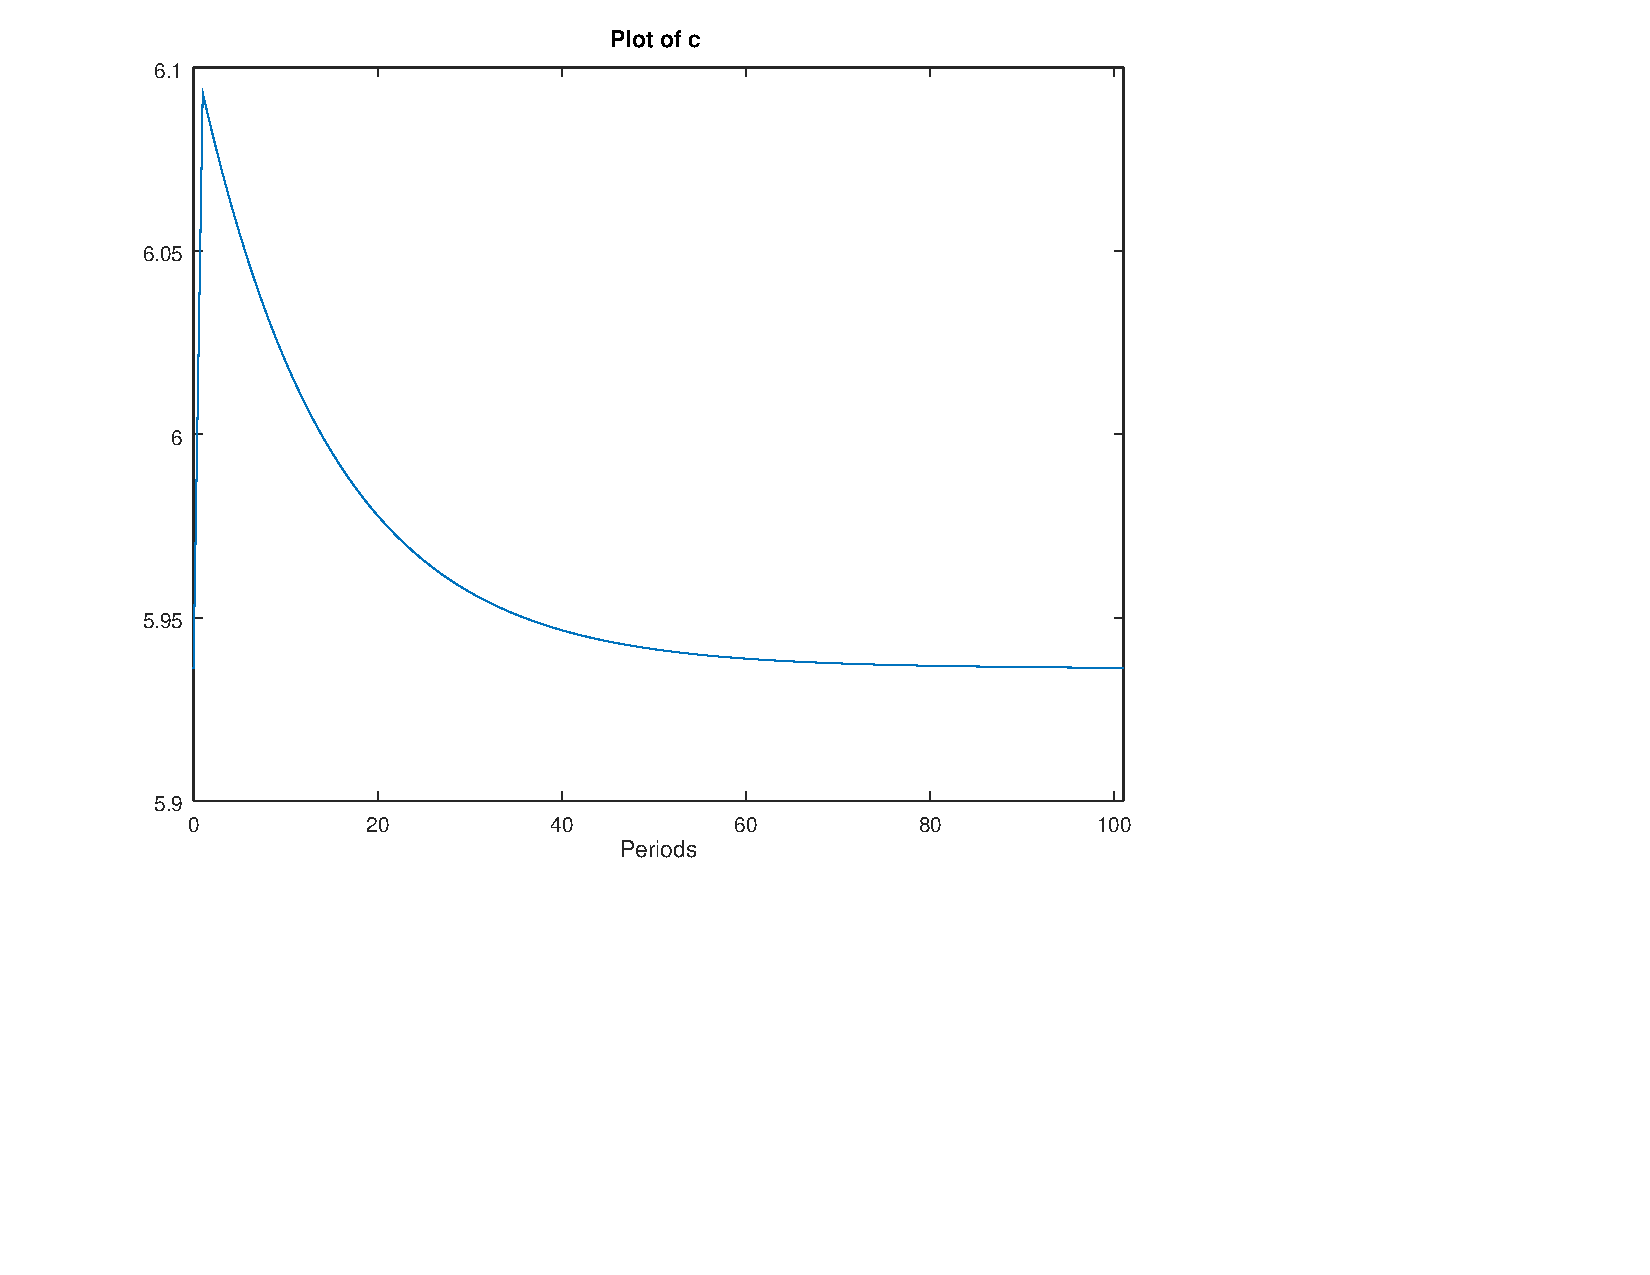
\includegraphics[width=15cm]{figures/rplot_c.pdf}
\end{frame}


\begin{frame}
  \frametitle{The general problem}
  \begin{witemize}
    \item Perfect foresight problem can be represented as
    \begin{equation}
      f(y_{t+1},y_t,y_{t-1},u_t)=0 ,
    \end{equation}
    with
    \begin{itemize}
      \item $y$: vector of endogenous variables
      \item $u$: vector of exogenous variables/shocks
    \end{itemize}

    \item Model requires a many endogenous variables $y$ as equations in $f$

  \end{witemize}
\end{frame}

\begin{frame}{Return to the neoclassical growth model}
  \begin{itemize}
    \item The neoclassical growth model has the representation:
          \begin{align}
            y_t                           & = \left(\begin{array}{c}
                                                        c_t \\
                                                        k_t
                                                      \end{array}
            \right)                                                                                                                           \\
            u_t                           & = A_t                                                                                             \\
            f(y_{t+1}, y_t, y_{t-1}, u_t) & = \left[\begin{array}{l}
                                                        c_t^{-\sigma} - \beta c_{t+1}^{-\sigma}\left(\alpha A_{t+1}k_t^{\alpha-1}+1-\delta\right) \\
                                                        c_t+k_t - A_t k_{t-1}^\alpha + (1-\delta)k_{t-1}
                                                      \end{array}\right]=0
          \end{align}

  \end{itemize}
\end{frame}

\begin{frame}
  \frametitle{Dealing with higher order leads and lags}

  \begin{witemize}
    \item Models can always be transformed to canonical form with at most one lead and lag using \textit{auxiliary} variables\\
    $\rightarrow$ transformation done automatically by Dynare
    \item Take variable with two leads $x_{t+2}$:
    \begin{itemize}
      \item create a new auxiliary variable $a$
      \item add a new equation: $a_t = x_{t+1}$
      \item replace all occurrences of $x_{t+2}$ by $a_{t+1}$
    \end{itemize}
    \item Symmetric process for variables with more than one lag
    \item With future uncertainty, transformation is more elaborate
    (but still possible) on variables with leads
    \item \texttt{write\_latex\_original\_model}  and \texttt{write\_latex\_dynamic\_model} show model before and after substitution
  \end{witemize}
\end{frame}


\begin{frame}{Steady state}
  \begin{witemize}
    \item A steady state $y$ for the model satisfies
    \begin{equation}
      f(y, y, y, u) = 0
    \end{equation}

    \item Note that, in this context, a steady state is conditional on
    \begin{witemize}
      \item steady state values of exogenous variables $u$
      \item structural parameters (implicit in $f$)
    \end{witemize}

    \item Careful: such a steady state may not be unique
    \item The steady state is computed/checked by Dynare with the \texttt{steady} command\\
    $\rightarrow$ triggers a nonlinear solver if no analytical steady state is provided
  \end{witemize}

\end{frame}


\begin{frame}
  \frametitle{Towards a solution}
  \begin{witemize}
    \item In each period, agent needs to choose consumption today, taking into account
    \begin{witemize}
      \item the known time path of the exogenous states
      \item the current endogenous states that cannot be altered anymore (capital)
      \item the consequences of today's actions for future decisions
    \end{witemize}
    \item Assume finite horizon problem that terminates in period $T$ with
    \begin{witemize}
      \item initial states in $y_0$ given
      \item terminal choice $y_{T+1}$ known
    \end{witemize}
    $\rightarrow$ problem boils down to simultaneous equation system with $n_y\times T$ equations in $n_y\times T$ unknowns
  \end{witemize}

\end{frame}

\begin{frame}{A two-boundary value problem}

  \begin{witemize}
    \item Problem can be formulated as stacked system over $T$ periods, given ${\red y_0}$ and ${\red y_{T+1}}$
    \begin{equation}
      \left\{\begin{array}{c}
        f(y_2,y_1,{\red y_0},u_1)=0 \\
        f(y_3,y_2,y_1,u_2)=0        \\
        \vdots                      \\
        f({\red y_{T+1}},y_T,y_{T-1},u_T)=0
      \end{array}\right.
    \end{equation}
    \item More compactly:
    \begin{equation}
      F(Y) = 0 \: ,
    \end{equation}
    where $Y =
      \left[\begin{array}{llll}y_1'&y_2'&\ldots&y_T'\end{array}\right]'$ and ``exogenous'' elements $y_0$, $y_{T+1}$, $u_1\ldots u_T$ are implicit
    \item Stacked equation system can be solved using a Newton-type method
  \end{witemize}
\end{frame}


\begin{frame}{Approximating infinite-horizon problems}
  \begin{witemize}
    \item What if you are interested in solving \emph{infinite}-horizon problem instead of \emph{finite}-horizon one?
    \item One option: compute recursive policy function (e.g.\
    perturbation), but this is challenging
    \begin{itemize}
      \item in general, this function is defined over infinite-dimensional space
            (all future shocks are state variables)
      \item in case of a return to equilibrium, state-space
            is finite (starting from date where all shocks are zero), but a
            projection method would still be needed
            $\rightarrow$ Dynare does not support this
    \end{itemize}
    \item Often easier way in case of return to equilibrium: approximate solution by a finite-horizon problem\\
    $\rightarrow$ computing the trajectory with $y_{T+1}=\bar y$ and $T$
    large enough
    \item Drawback compared to policy function approach: solution specific to a given sequence of shocks, and not generic
  \end{witemize}
\end{frame}

\section[Solution]{Solution techniques}

\begin{frame}
  \frametitle{The Newton method (unidimensional)}
  \medskip
  \only<1>{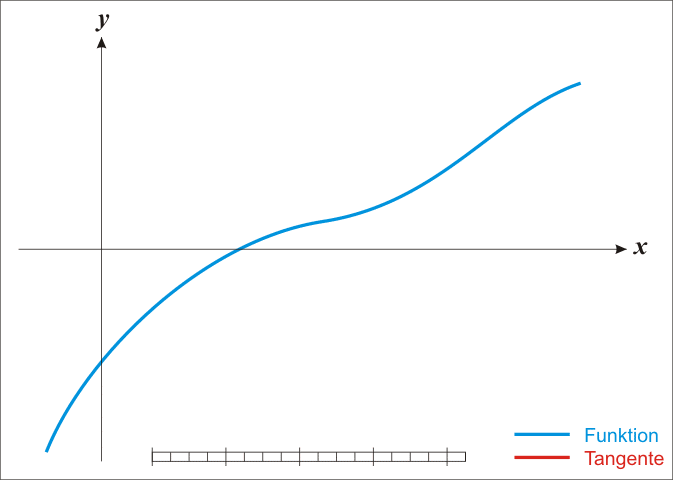
\includegraphics[width=10cm]{figures/NewtonIteration_Ani-0.png}}\only<2>{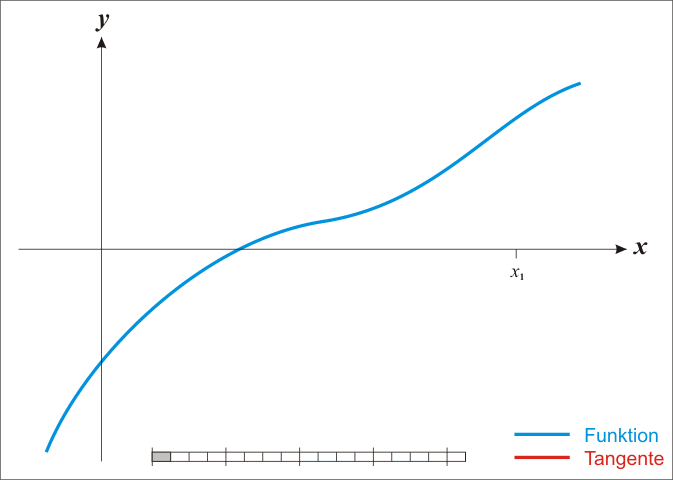
\includegraphics[width=10cm]{figures/NewtonIteration_Ani-1.png}}\only<3>{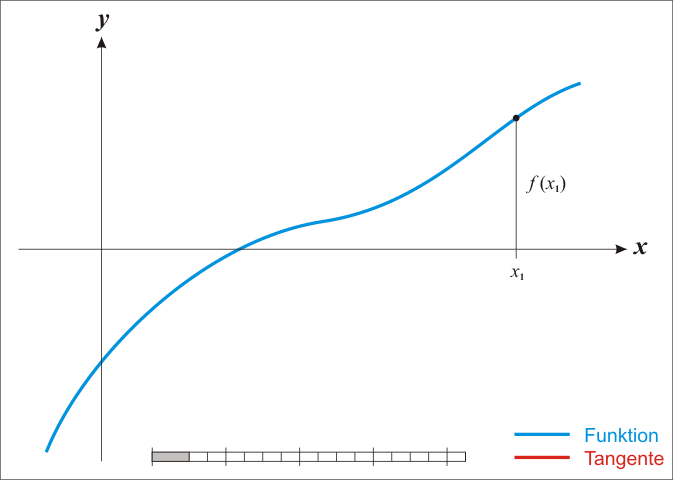
\includegraphics[width=10cm]{figures/NewtonIteration_Ani-2.png}}\only<4>{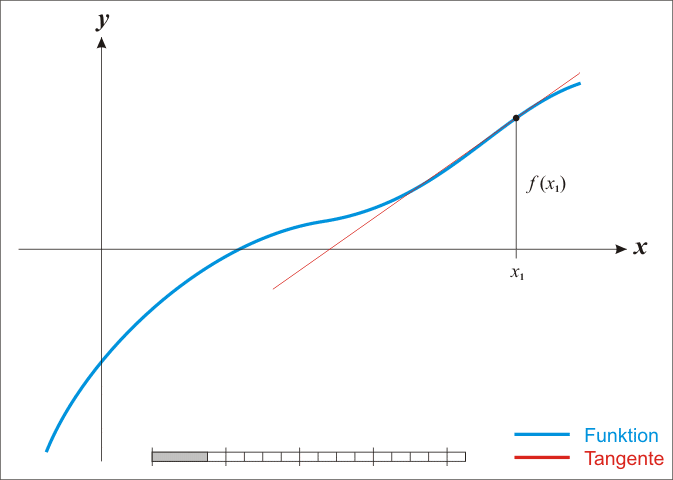
\includegraphics[width=10cm]{figures/NewtonIteration_Ani-3.png}}\only<5>{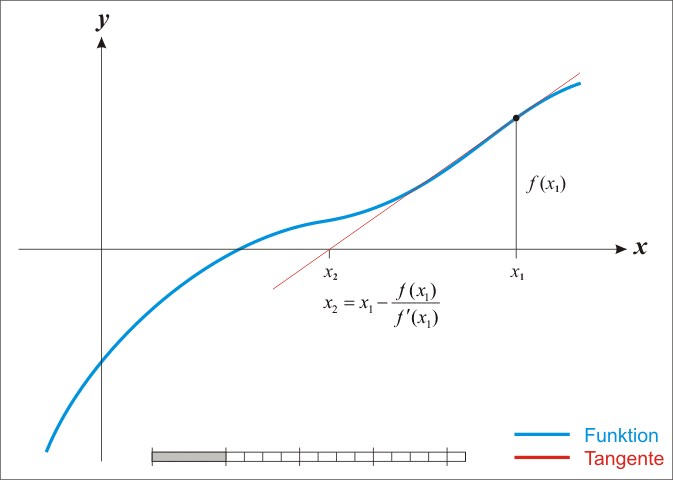
\includegraphics[width=10cm]{figures/NewtonIteration_Ani-4.png}}\only<6>{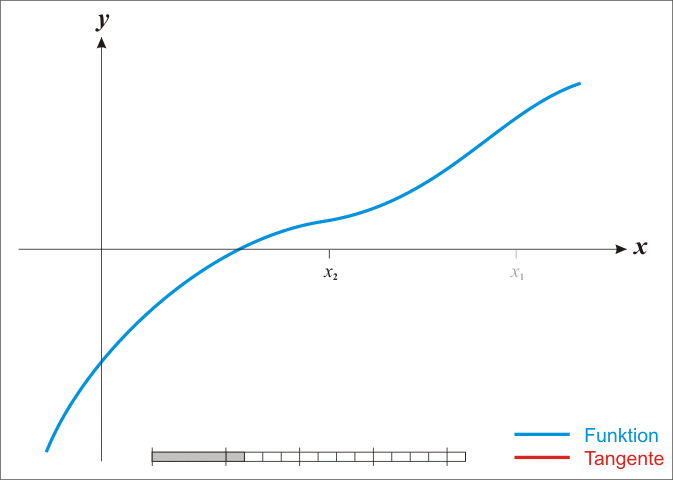
\includegraphics[width=10cm]{figures/NewtonIteration_Ani-5.png}}\only<7>{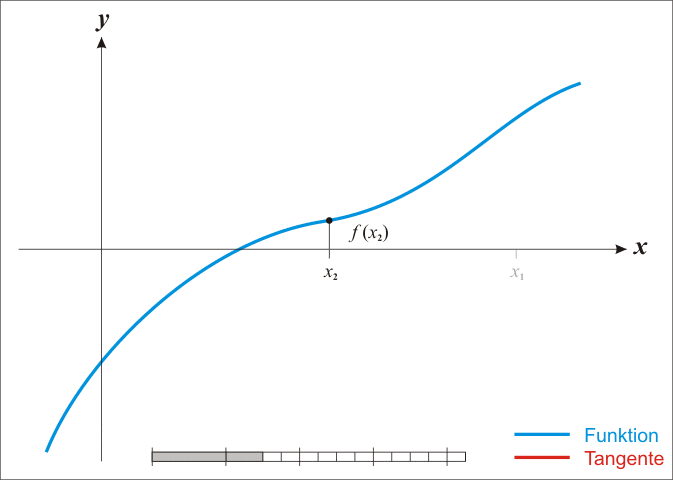
\includegraphics[width=10cm]{figures/NewtonIteration_Ani-6.png}}\only<8>{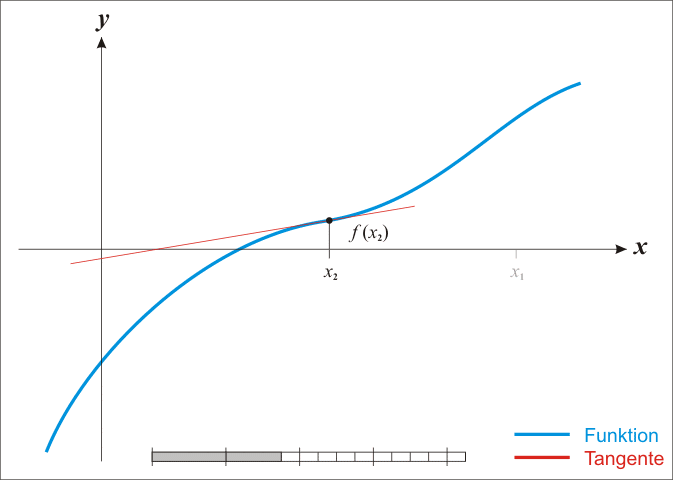
\includegraphics[width=10cm]{figures/NewtonIteration_Ani-7.png}}\only<9>{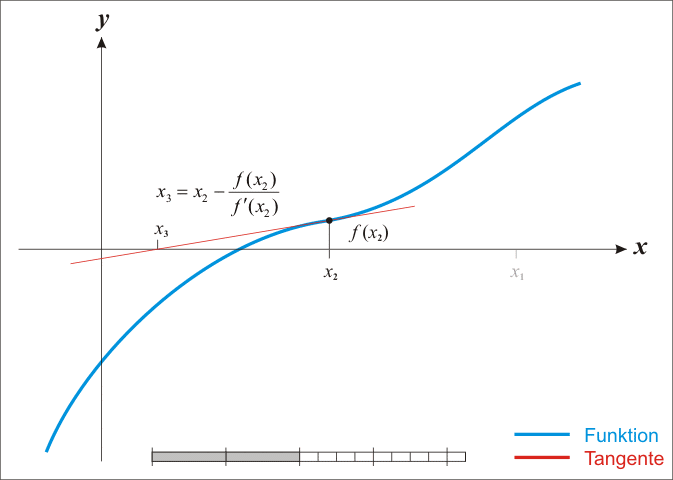
\includegraphics[width=10cm]{figures/NewtonIteration_Ani-8.png}}\only<10>{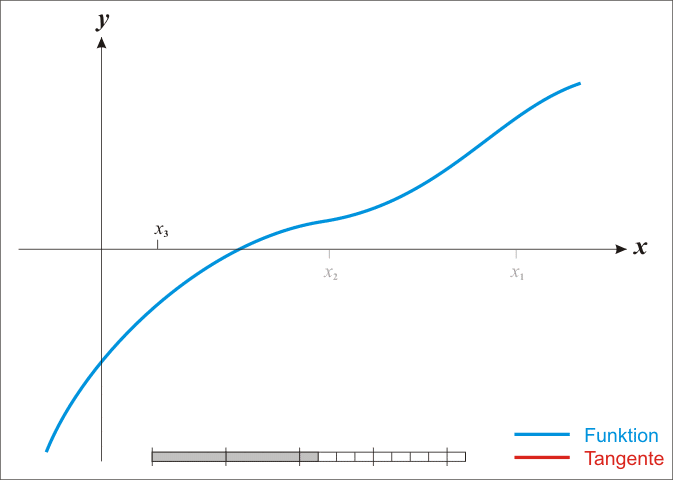
\includegraphics[width=10cm]{figures/NewtonIteration_Ani-9.png}}\only<11>{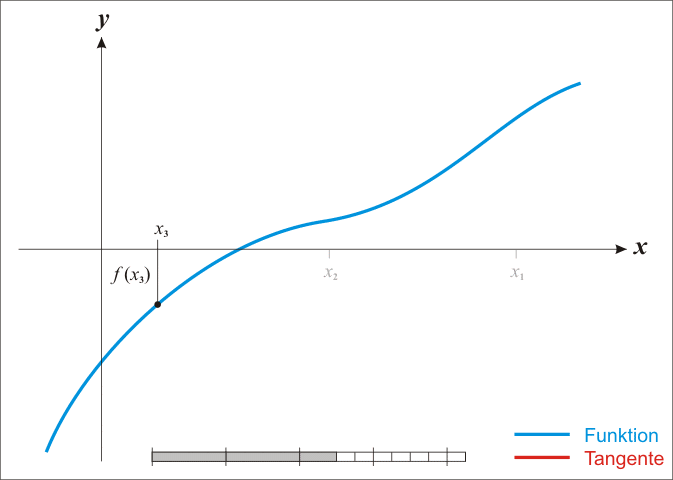
\includegraphics[width=10cm]{figures/NewtonIteration_Ani-10.png}}\only<12>{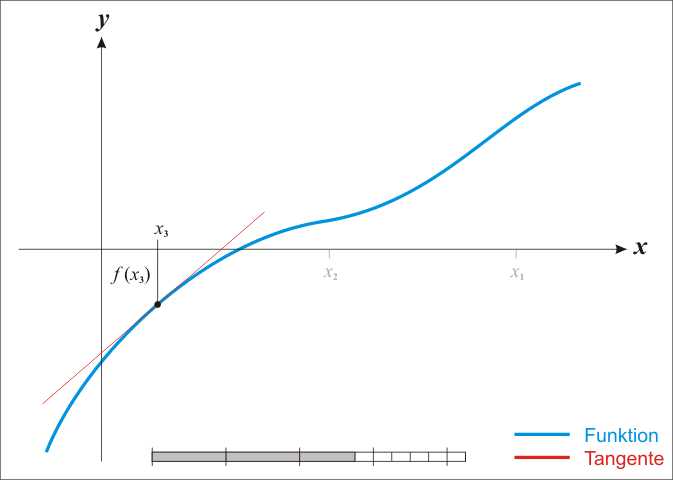
\includegraphics[width=10cm]{figures/NewtonIteration_Ani-11.png}}\only<13>{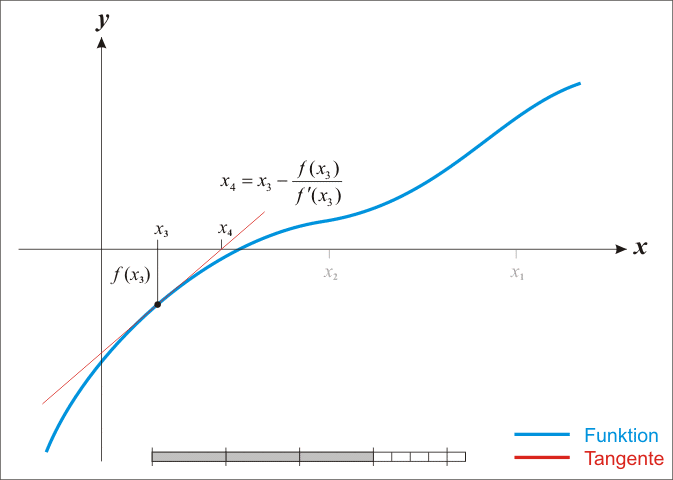
\includegraphics[width=10cm]{figures/NewtonIteration_Ani-12.png}}\only<14>{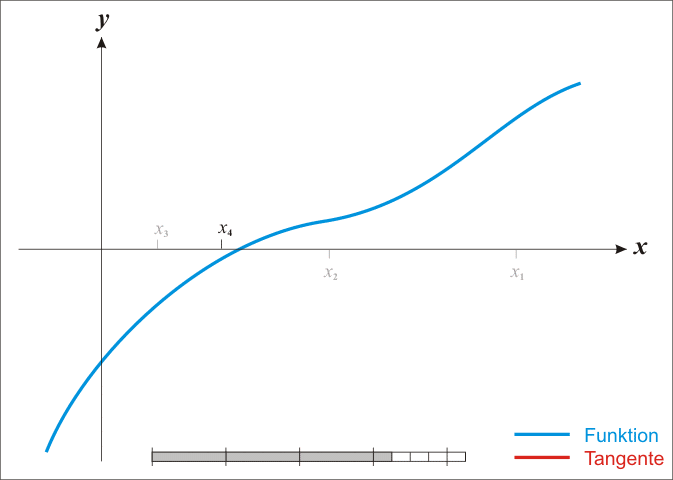
\includegraphics[width=10cm]{figures/NewtonIteration_Ani-13.png}}\only<15>{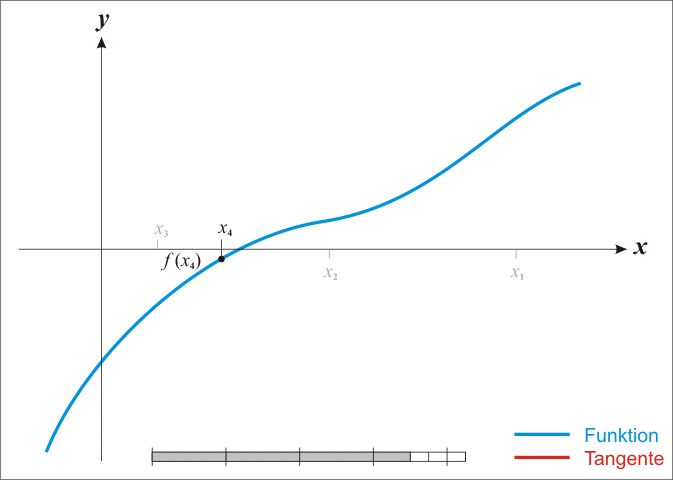
\includegraphics[width=10cm]{figures/NewtonIteration_Ani-14.png}}\only<16>{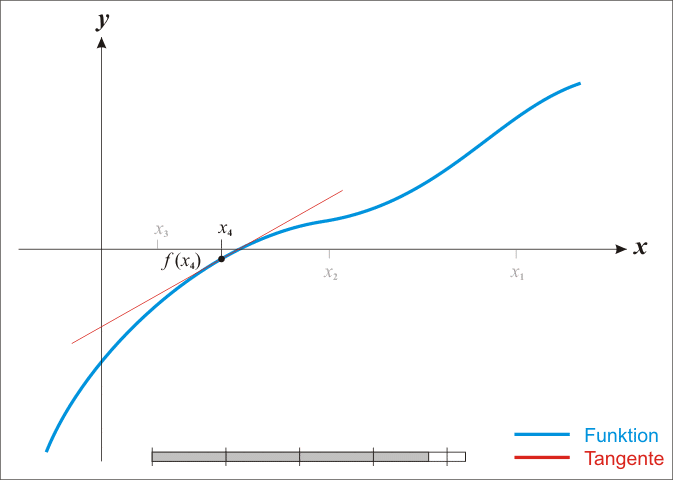
\includegraphics[width=10cm]{figures/NewtonIteration_Ani-15.png}}\only<17>{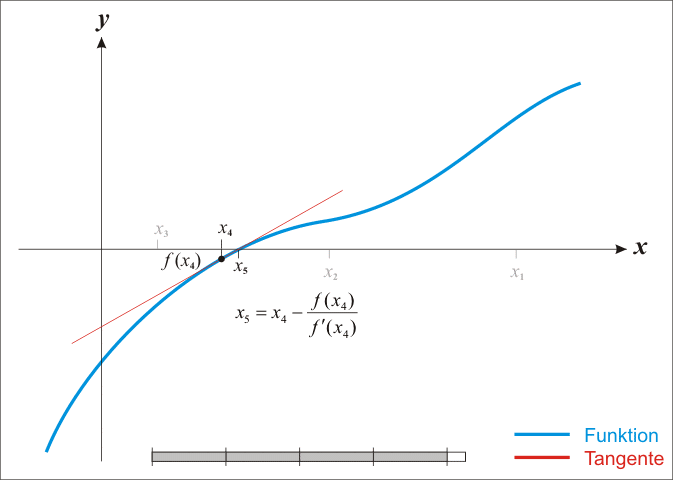
\includegraphics[width=10cm]{figures/NewtonIteration_Ani-16.png}}\only<18>{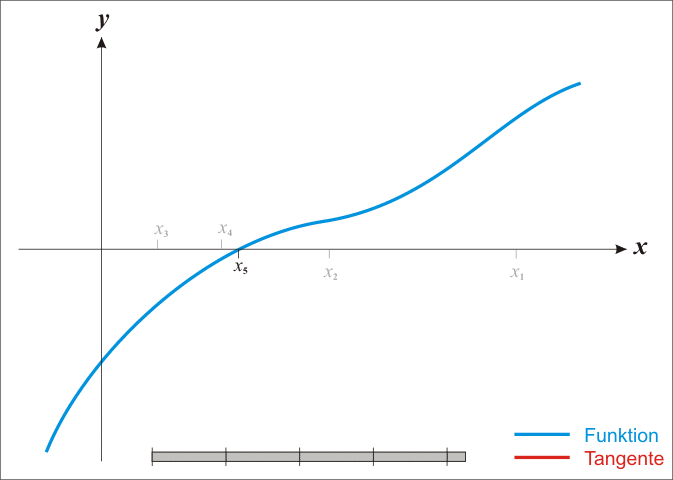
\includegraphics[width=10cm]{figures/NewtonIteration_Ani-17.png}}

  {\vspace*{-2mm} \tiny Copyright © 2005 Ralf Pfeifer / \href{http://creativecommons.org/licenses/by-sa/3.0/}{Creative Commons Attribution-ShareAlike 3.0}}
\end{frame}

\begin{frame}\frametitle{The Newton method (multidimensional)}
  \begin{witemize}
    \item Start from an initial guess $Y^{(0)}$
    \item Iterate with updated solutions $Y^{(k+1)}$ obtained by solving linear
    system:
    \begin{equation}
      F(Y^{(k)}) + \left[\frac{\partial F}{\partial Y}\right]\left(Y^{(k+1)}
      -Y^{(k)}\right) = 0
    \end{equation}
    \item Terminate if problem solved or no more improvement:
    \begin{equation}
      ||F(Y^{(k)})||_\infty <
      \varepsilon_F \qquad \text{or} \qquad  ||Y^{(k+1)}-Y^{(k)}||_\infty < \varepsilon_Y
    \end{equation}
    \item Convergence may never happen if function is ill-behaved or initial guess $Y^{(0)}$ too far
    from a solution \\
    $\rightarrow$ to avoid an infinite loop, abort after a given number of iterations
  \end{witemize}
\end{frame}

\begin{frame}
  \frametitle{Controlling the Newton algorithm from Dynare}
  The following options to the \texttt{perfect\_foresight\_solver} can be used
  to control the Newton algorithm:
  \begin{description}
    \item[\texttt{maxit}] Maximum number of iterations before aborting (default: 50)

    \item[\texttt{tolf}] Convergence criterion based on function value ($\varepsilon_F$)
          (default: $10^{-5}$)
    \item[\texttt{tolx}] Convergence criterion based on change in the function argument ($\varepsilon_Y$)
          (default: $10^{-5}$)
    \item[\texttt{stack\_solve\_algo}] selects between the different flavors of Newton
          algorithms (more later)
  \end{description}
\end{frame}

\begin{frame}
  \frametitle{A practical difficulty}
  \begin{witemize}
    \item   Jacobian matrix of dimension $n_yT\times n_yT$ can be really large!
    \item Three alternative ways of dealing with large problem size:
    \begin{wenumerate}
      \item Exploit particular structure of Jacobian using a technique
      developed by \textcite{Laffargue1990}, \textcite{Boucekkine1995} and \textcite{Juillard1996} (was the default method in
      Dynare $\leq$ 4.2)
      \item Handle the Jacobian as one large sparse matrix (now the default method)
      \item Dulmage/Mendelsohn block decomposition, which is a divide-and-conquer method (can be combined with one of the previous two methods)\\
      $\rightarrow$ will be the default in Dynare 7
    \end{wenumerate}
  \end{witemize}
\end{frame}

\begin{frame}
  \frametitle{Shape of the Jacobian}
  \begin{equation}
    \frac{\partial F}{\partial Y} = \begin{pmatrix}
      B_1 & C_1    &        &        &         &         &         \\
      A_2 & B_2    & C_2    &        &         &         &         \\
          & \ddots & \ddots & \ddots &         &         &         \\
          &        & A_t    & B_t    & C_t     &         &         \\
          &        &        & \ddots & \ddots  & \ddots  &         \\
          &        &        &        & A_{T-1} & B_{T-1} & C_{T-1} \\
          &        &        &        &         & A_T     & B_T
    \end{pmatrix}
  \end{equation}

  \begin{align}
    A_s & = \frac{\partial f}{\partial y_{t-1}}(y_{s+1},y_s,y_{s-1}) \\
    B_s & = \frac{\partial f}{\partial y_t}(y_{s+1},y_s,y_{s-1})     \\
    C_s & = \frac{\partial f}{\partial y_{t+1}}(y_{s+1},y_s,y_{s-1})
  \end{align}
\end{frame}



\begin{frame}
  \frametitle{Laffargue-Boucekkine-Juillard algorithm (1/5)}
  \begin{itemize}
    \item  The idea is to triangularize the stacked system:
          \begin{small}
            \begin{equation}
              \begin{pmatrix}
                B_1 & C_1    &        &         &         &         \\
                A_2 & B_2    & C_2    &         &         &         \\
                    & \ddots & \ddots & \ddots  &         &         \\
                    &        & \ddots & \ddots  & \ddots  &         \\
                    &        &        & A_{T-1} & B_{T-1} & C_{T-1} \\
                    &        &        &         & A_T     & B_T
              \end{pmatrix}
              \Delta Y
              =
              -\begin{pmatrix}
                f(y_2,y_1,y_0,u_1)             \\
                f(y_3,y_2,y_1,u_2)             \\
                \vdots                         \\
                \vdots                         \\
                f(y_{T},y_{T-1},y_{T},u_{T-1}) \\
                f(y_{T+1},y_T,y_{T-1},u_T)
              \end{pmatrix} \: ,
            \end{equation}
          \end{small}
          eliminating elements below the main diagonal by proceeding recursively from the top
  \end{itemize}
\end{frame}


\begin{frame}
  \frametitle{Laffargue-Boucekkine-Juillard algorithm (2/5)}
  \begin{itemize}
    \item The first period is special due to the initial condition:
          \begin{small}
            \begin{equation}
              \begin{pmatrix}
                I & D_1        &        &         &         &         \\
                  & B_2-A_2D_1 & C_2    &         &         &         \\
                  & A_3        & B_3    & C_3     &         &         \\
                  &            & \ddots & \ddots  & \ddots  &         \\
                  &            &        & A_{T-1} & B_{T-1} & C_{T-1} \\
                  &            &        &         & A_T     & B_T
              \end{pmatrix}
              \Delta Y
              =
              -\begin{pmatrix}
                d_1                            \\
                f(y_3,y_2,y_1,u_2)+A_2 d_1     \\
                f(y_4,y_3,y_2,u_3)             \\
                \vdots                         \\
                f(y_{T},y_{T-1},y_{T},u_{T-1}) \\
                f(y_{T+1},y_T,y_{T-1},u_T)
              \end{pmatrix} \: ,
            \end{equation}
          \end{small}

          where

          \begin{itemize}
            \item $D_1 = B_1^{-1}C_1$
            \item $d_1 = B_1^{-1}f(y_2,y_1,y_0,u_1)$
          \end{itemize}
  \end{itemize}
\end{frame}

\begin{frame}
  \frametitle{Laffargue-Boucekkine-Juillard algorithm (3/5)}
  \begin{itemize}
    \item Normal iteration of the triangularization:
          \begin{small}
            \begin{equation}
              \begin{pmatrix}
                I & D_1 &            &         &         &         \\
                  & I   & D_2        &         &         &         \\
                  &     & B_3-A_3D_2 & C_3     &         &         \\
                  &     & \ddots     & \ddots  & \ddots  &         \\
                  &     &            & A_{T-1} & B_{T-1} & C_{T-1} \\
                  &     &            &         & A_T     & B_T
              \end{pmatrix}
              \Delta Y
              =
              -\begin{pmatrix}
                d_1                            \\
                d_2                            \\
                f(y_4,y_3,y_2,u_3) + A_3d_2    \\
                \vdots                         \\
                f(y_{T},y_{T-1},y_{T},u_{T-1}) \\
                f(y_{T+1},y_T,y_{T-1},u_T)
              \end{pmatrix} \: ,
            \end{equation}
          \end{small}

          where

          \begin{itemize}
            \item $D_2 = (B_2-A_2D_1)^{-1}C_2$
            \item $d_2 = (B_2-A_2D_1)^{-1}(f(y_3,y_2,y_1,u_2)+A_2d_1)$
          \end{itemize}
  \end{itemize}
\end{frame}

\begin{frame}
  \frametitle{Laffargue-Boucekkine-Juillard algorithm (4/5)}
  \begin{itemize}
    \item Final iteration:
          \begin{small}
            \begin{equation}
              \begin{pmatrix}
                I & D_1 &     &        &        &         \\
                  & I   & D_2 &        &        &         \\
                  &     & I   & D_3    &        &         \\
                  &     &     & \ddots & \ddots &         \\
                  &     &     &        & I      & D_{T-1} \\
                  &     &     &        &        & I
              \end{pmatrix}
              \Delta Y
              =
              -\begin{pmatrix}
                d_1     \\
                d_2     \\
                d_3     \\
                \vdots  \\
                d_{T-1} \\
                d_T
              \end{pmatrix}
            \end{equation}
          \end{small}
          where
          \begin{equation}
            d_T = (B_T-A_TD_{T-1})^{-1}(f(y_{T+1},y_T,y_{T-1},u_T)+A_Td_{T-1})
          \end{equation}
  \end{itemize}
\end{frame}

\begin{frame}
  \frametitle{Laffargue-Boucekkine-Juillard algorithm (5/5)}
  \begin{itemize}
    \item The triangular system can then solved by backward iteration:
          \begin{align}
            y_T^{k+1}     & = y_T^k - d_T                                      \\
            y_{T-1}^{k+1} & = y_{T-1}^k - d_{T-1} - D_{T-1}(y_T^{k+1} - y_T^k) \\
                          & \vdots                                             \\
            y_1^{k+1}     & = y_1^k - d_1 - D_1(y_2^{k+1} - y_2^k)
          \end{align}

    \item Advantage: no need to ever store the whole Jacobian, only the $D_s$ and $d_s$ \\
          $\rightarrow$ memory efficiency made it default method in Dynare $\leq$ 4.2
    \item Still available as option \texttt{stack\_solve\_algo=6} of
          \texttt{perfect\_foresight\_solver} command (or
          \texttt{stack\_solve\_algo=1} in Dynare 6)
  \end{itemize}
\end{frame}

\begin{frame}
  \frametitle{Sparse matrices (1/3)}
  \begin{witemize}
    \item Consider the following matrix with most elements equal to zero:
    \begin{equation}
      A = \left(\begin{matrix}
        0  & 0 & 2.5 \\
        -3 & 0 & 0   \\
        0  & 0 & 0
      \end{matrix}\right)
    \end{equation}
    \item Dense matrix storage (in column-major order) treats it as a
    one-dimensional array: $$[0, -3, 0, 0, 0, 0, 2.5, 0, 0]$$
    \item Sparse matrix storage:
    \begin{itemize}
      \item views it as a list of triplets $(i,j,v)$ where
            $(i,j)$ is a matrix coordinate and $v$ a non-zero value
      \item $A$ would be stored as $$\{(2,1,-3), (1,3,2.5)\}$$
    \end{itemize}
  \end{witemize}
\end{frame}

\begin{frame}
  \frametitle{Sparse matrices (2/3): memory considerations}
  \begin{witemize}
    \item In the general case, given an $m\times n$ matrix with $k$ non-zero
    elements:
    \begin{witemize}
      \item dense matrix storage = $8mn$ bytes
      \item sparse matrix storage = $16k$ bytes
      \item sparse storage more memory-efficient as soon as $k < mn/2$
    \end{witemize}
    (assuming 32-bit integers and 64-bit floating point numbers)
    \item In practice, sparse storage becomes interesting if $k \ll mn/2$, because
    linear algebra algorithms are vectorized
  \end{witemize}
\end{frame}

\begin{frame}
  \frametitle{Sparse matrices (3/3): DSGE models}
  \begin{witemize}
    \item The Jacobian of the deterministic problem is a sparse matrix:
    \begin{itemize}
      \item Lots of zero blocks
      \item The $A_s$, $B_s$ and $C_s$ usually are themselves sparse
    \end{itemize}
    \item Many optimized algorithms for sparse matrices exist, including solver for linear equation solving in Newton algorithm
    \item Sparse matrices exist as native objects in MATLAB/Octave (see \texttt{sparse} command)
    \item Works well for medium-size deterministic models
    \item Nowadays more efficient than Laffargue-Boucekkine-Juillard, despite not exploiting the particular structure of the Jacobian \\
    $\Rightarrow$ current default method in Dynare 6 (\texttt{stack\_solve\_algo=0})

  \end{witemize}

\end{frame}


\begin{frame}
  \frametitle{Block decomposition (1/3): idea}
  \begin{witemize}
    \item Idea: apply a divide-and-conquer technique to model simulation\\
    $\rightarrow$ block triangularization of the Jacobian
    \item Principle: identify recursive as well as simultaneous blocks in the model structure
    \begin{enumerate}
      \item First block (prologue): equations that only involve variables
            determined by previous equations\\
            $\rightarrow$  e.g. $AR(1)$ processes
      \item Last block (epilogue): pure output/reporting equations
      \item In between: simultaneous blocks that depend recursively on each other
    \end{enumerate}
    \item Identification of blocks and block types is performed through matching between variables and equations (normalization), then reordering both
  \end{witemize}
\end{frame}

\begin{frame}
  \frametitle{Block decomposition (2/3)}
  \framesubtitle{Form of the reordered Jacobian (equations in lines, variables
    in columns)}
  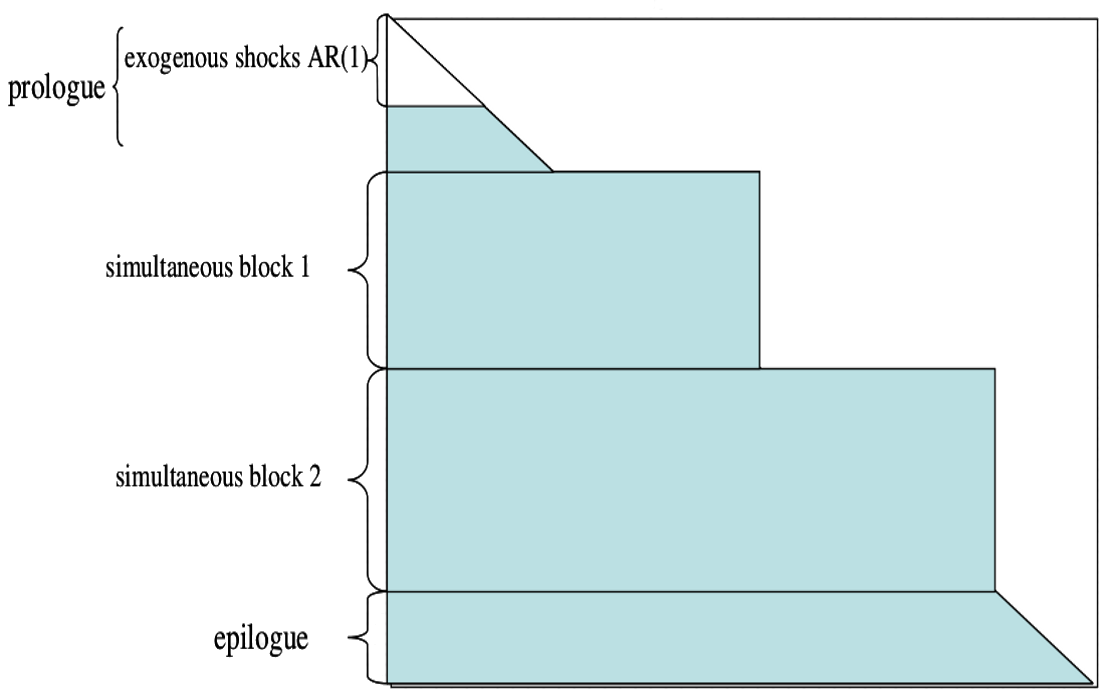
\includegraphics[width=11cm]{figures/block.png}
\end{frame}

\begin{frame}
  \frametitle{Block decomposition (3/3)}
  \begin{witemize}
    \item Can provide significant speed-up on large models
    \item Implemented in Dynare by Ferhat Mihoubi
    \item Available as option \texttt{block} to the \texttt{model} command
    \item Bigger gains when used in conjunction with \texttt{bytecode} or \texttt{use\_dll}  option
    \item Can be combined with any flavor of the Newton method applied to each
    individual block
  \end{witemize}
\end{frame}

\begin{frame}
  \frametitle{Homotopy}
  \begin{itemize}
    \item Another divide-and-conquer method, but in the shocks dimension
    \item Useful if large shocks prevent convergence
    \item Idea: achieve convergence for smaller shocks, use result as
          initial guess for bigger shock
    \item Algorithm:
          \begin{enumerate}
            \item $\lambda\leftarrow 0$: scaling factor of shocks (simulation succeeds when
                  $\lambda=1$)

            \item $s \leftarrow 1$: step size
            \item \label{loop} Try to compute simulation with shock scaling factor equal to
                  $\lambda + s$, using last successful computation as initial guess (with initial steady state at all $t$ as initial guess)
                  \begin{itemize}
                    \item If success: $\lambda \leftarrow (\lambda+s)$. Stop if $\lambda=1$.
                          Otherwise possibly increase $s$.
                    \item If failure: diminish $s$.
                  \end{itemize}
            \item Go to \ref{loop}
          \end{enumerate}
    \item Works with both temporary and permanent shocks (\textit{i.e.}
          \texttt{shocks} and \texttt{endval})
    \item Can be combined with any deterministic solver
    \item Enabled by default in \texttt{perfect\_foresight\_solver} (disable with
          option \texttt{no\_homotopy})
  \end{itemize}
\end{frame}

\section[Shock types]{Shocks: temporary/permanent, unexpected/pre-announced}

\begin{frame}
  \frametitle{Example: neoclassical growth model with investment}
  The social planner problem is as follows:
  \begin{equation}
    \label{eq:social-planner-problem:1}
    \max_{\{c_{t},\ell_{t},k_{t}\}_{t=1}^{\infty}}
    \sum_{t=1}^{\infty}\beta^{t-1}u(c_{t},\ell_{t})
  \end{equation}
  s.t.
  \begin{align}
    y_t + (1-\delta)k_{t-1} & = c_t + k_t                           \\
    y_t                     & = A_tf(k_{t-1},\ell_t)                \\
    A_{t}                   & = {A^{\star}}e^{a_{t}}                \\
    a_{t}                   & = \rho\, a_{t-1} + \varepsilon_t \: ,
  \end{align}
  where $\varepsilon_t$ is an exogenous shock and $k_0$ given.
\end{frame}

\begin{frame}
  \frametitle{Functional forms}
  \begin{itemize}
    \item Utility function is non-separable:
          \begin{equation}
            u(c_t,\ell_t) = \frac{\left(c_t^{\theta}(1-\ell_t)^{1-\theta}\right)^{1-\tau}}{1-\tau}
          \end{equation}

    \item CES production function:
          \begin{equation}
            f(k_{t-1},\ell_t) = \left(\alpha k_{t-1}^{\psi} + (1-\alpha)\ell_t^{\psi}\right)^{\frac{1}{\psi}}
          \end{equation}
  \end{itemize}
\end{frame}

\begin{frame}
  \frametitle{First order conditions}
  \begin{itemize}
    \item Euler equation:
          \begin{equation}
            u_c(c_t,\ell_t) = \beta\, \mathbb E_t\left[
              u_c(c_{t+1},\ell_{t+1})\Bigl(A_{t+1}f_k(k_t,\ell_{t+1}) + 1
              -\delta\Bigr) \right]
          \end{equation}
    \item Consumption/leisure tradeoff:
          \begin{equation}
            \frac{u_{\ell}(c_t,\ell_t)}{u_c(c_t,\ell_t)} + A_t f_{\ell}(k_{t-1},\ell_t) = 0
          \end{equation}
    \item Resource constraint:
          \begin{equation}
            c_t + k_t = A_tf(k_{t-1},\ell_t) + (1-\delta)k_{t-1}
          \end{equation}
  \end{itemize}
\end{frame}


\begin{frame}[fragile]{Dynare code (1/3)}{\texttt{rbc\_det1.mod}}
  \begin{minted}{c++}
var k, y, L, c, A, a;
varexo epsilon;
parameters beta, theta, tau, alpha, psi, delta, rho, Astar;

beta = 0.99;
theta = 0.357;
tau = 2;
alpha = 0.45;
psi = -0.1;
delta = 0.02;
rho = 0.8;
Astar = 1;
\end{minted}
\end{frame}

\begin{frame}[fragile]{Dynare code (2/3)}{\texttt{rbc\_det1.mod}}
  \begin{minted}{c++}
model;
  a = rho*a(-1) + epsilon;
  A = Astar*exp(a);
  y = A*(alpha*k(-1)^psi+(1-alpha)*L^psi)^(1/psi);
  k = y-c + (1-delta)*k(-1);
  (1-theta)/theta*c/(1-L) - (1-alpha)*(y/L)^(1-psi);
  (c^theta*(1-L)^(1-theta))^(1-tau)/c =
     beta*(c(+1)^theta*(1-L(+1))^(1-theta))^(1-tau)/c(+1)
      *(alpha*(y(+1)/k)^(1-psi)+1-delta);
end;
\end{minted}
\end{frame}

\begin{frame}[fragile,fragile]{Dynare code (3/3)}
  %\scriptsize
  \begin{minted}{c++}
steady_state_model;
  a = epsilon/(1-rho);
  A = Astar*exp(a);
  y_over_k=((1/beta-1+delta)/alpha)^(1/(1-psi));
  c_over_k=y_over_k-delta;
  l_over_k=(((y_over_k/A)^psi-alpha)/(1-alpha))^(1/psi);
  y_over_l=y_over_k/l_over_k;
  c_over_l=c_over_k/l_over_k;

  % Compute steady state of the endogenous variables.
  L=1/(1+c_over_l/((1-alpha)*theta/(1-theta)*y_over_l^(1-psi)));
  c=c_over_l*L;
  k=L/l_over_k;
  y=y_over_k*k;
end;
\end{minted}
\end{frame}



\begin{frame}[fragile]{Scenario 1: Return to equilibrium}{\texttt{rbc\_det1.mod}}
  Return to equilibrium starting from $k_0 = 0.5 \bar k$.

  \begin{minted}{c++}
...
steady;

ik = varlist_indices('k',M_.endo_names);
kstar = oo_.steady_state(ik);

histval;
  k(0) = kstar/2;
end;

perfect_foresight_setup(periods=300);
perfect_foresight_solver;
\end{minted}
\end{frame}

\begin{frame}[fragile]{Scenario 2: A temporary shock to TFP}{\texttt{rbc\_det2.mod}}
  \begin{itemize}
    \item Economy starts from steady state
    \item At beginning of period 1: unexpected negative shock $\varepsilon_1=-0.1$
  \end{itemize}

  \begin{minted}{c++}
...
steady;

shocks;
  var epsilon;
  periods 1;
  values -0.1;
end;

perfect_foresight_setup(periods=300);
perfect_foresight_solver;
\end{minted}
\end{frame}

\begin{frame}[fragile]{Scenario 3: Pre-announced  favorable shocks in the future}{\texttt{rbc\_det3.mod}}
  \begin{itemize}
    \item Economy starts from steady state
    \item Sequence of positive shocks to $A_t$: 4\% in period 5 and additional 1\% during the 4 following periods
  \end{itemize}

  \begin{minted}{c++}
...
steady;

shocks;
  var epsilon;
  periods 4, 5:8;
  values 0.04, 0.01;
end;

perfect_foresight_setup(periods=300);
perfect_foresight_solver;
\end{minted}
\end{frame}

\begin{frame}[fragile]{Scenario 4: A permanent shock}{\texttt{rbc\_det4.mod}}
  \begin{itemize}
    \item Economy starts from the initial steady state ($a_0=0$)
    \item Period 1: TFP permanently increases by 5\% (and this was unexpected)
  \end{itemize}

  \begin{minted}{c++}
...
initval;
  epsilon = 0;
end;

steady;

endval;
  epsilon = (1-rho)*log(1.05);
end;

steady;
\end{minted}
\end{frame}

\begin{frame}[fragile]{Scenario 5: A pre-announced permanent shock}{\texttt{rbc\_det5.mod}}
  \begin{itemize}
    \item Economy starts from initial steady state ($a_0=0$)
    \item Period 6: TFP permanently increases by 5\%
    \item A \texttt{shocks;} block is used to maintain TFP at initial level
          during periods 1--5
  \end{itemize}

  \begin{minted}{c++}
...
// Same initval and endval blocks as in Scenario 4
...

shocks;
  var epsilon;
  periods 1:5;
  values 0;
end;
\end{minted}
\end{frame}

\begin{frame}
  \frametitle{Summary of commands}
  \begin{witemize}
    \item[1.] Only \texttt{initval} or \texttt{endval} followed by \texttt{steady}: set initial and terminal steady state
    \item[2.] \texttt{histval} for initial state variable conditions out of steady
    state\\
    $\rightarrow$ \texttt{initval} followed by \texttt{steady} for terminal steady state
    \item[3.] \texttt{initval} for initial condition (potentially followed by \texttt{steady}) and \texttt{endval} followed by \texttt{steady} for the terminal steady state
    \item \texttt{shocks;} block for shocks along the simulation path
    \item \texttt{perfect\_foresight\_setup} prepares the simulation
    \item \texttt{perfect\_foresight\_solver} computes the simulation
  \end{witemize}
\end{frame}

\begin{frame}
  \frametitle{Under the hood}
  \begin{witemize}
    \item Paths for exogenous and endogenous variables are stored in two
    MATLAB/Octave matrices:
    \begin{equation*}
      \begin{matrix}
        \texttt{oo\_.endo\_simul}                & = & ( & y_0       & y_1 & \ldots & y_T & y_{T+1}   & ) \\
        \texttt{oo\_.exo\_simul\textquotesingle} & = & ( & \boxtimes & u_1 & \ldots & u_T & \boxtimes & )
      \end{matrix}
    \end{equation*}
    \item for historical reasons, dates are in columns in
    \texttt{oo\_.endo\_simul} and in lines in \\
    \texttt{oo\_.exo\_simul},
    hence the transpose (\texttt{\textquotesingle})
    \item If there are exogenous leads/lags, $u_0$ and/or $u_{T+1}$ would be in \texttt{oo\_.exo\_simul\textquotesingle} as well\\
    $\rightarrow$ more leads/lags would show up as auxiliary variables

    \item \texttt{perfect\_foresight\_setup} initializes those
    matrices, given the \texttt{shocks}, \texttt{initval}, \texttt{endval}, and
    \texttt{histval} blocks
    \begin{itemize}
      \item $y_0$, $y_{T+1}$ and $u_1 \ldots u_T$ are the constraints of the
            problem
      \item $y_1\ldots y_T$ are the initial guess for the Newton algorithm
    \end{itemize}
    \item \texttt{perfect\_foresight\_solver} replaces $y_1\ldots y_T$ in
    \texttt{oo\_.endo\_simul} by the solution
  \end{witemize}
\end{frame}

\begin{frame}
  \frametitle{Initial guess}
  \begin{witemize}
    \item  The Newton algorithm needs an initial guess $Y^{(0)}= [ {y_1^{(0)}}'\;\ldots\;
      {y_T^{(0)}}' ]$.
    \item Dynare uses content of \texttt{oo\_.endo\_simul} created by \texttt{perfect\_foresight\_setup}
    \begin{itemize}
      \item without \texttt{endval}, it is steady state as specified by \texttt{initval} (repeated for all simulations periods)
      \item with \texttt{endval}, it is the terminal steady state declared within this block
    \end{itemize}
    \item Opens possibility of manipulating
    \texttt{oo\_.endo\_simul} after \texttt{perfect\_foresight\_setup} (but of
    course before \texttt{perfect\_foresight\_solver}!)
    \item If \texttt{homotopy} is triggered, initial guess of subsequent iterations
    is result of previous iteration
  \end{witemize}
\end{frame}

\begin{frame}
  \frametitle{Alternative way of specifying terminal conditions}
  \begin{witemize}
    \item What if
    \begin{itemize}
      \item final steady state is hard to compute?
      \item model is very persistent and takes a long time to go back to steady
            state?
    \end{itemize}
    \item \texttt{differentiate\_forward\_vars} option of \texttt{model} block allows computing terminal condition endogenously and avoiding final kink if
    $T$ is not large enough
    \item This is achieved by substituting for forward-looking variables using new auxiliary variables:
    \begin{itemize}
      \item Substitution: $x_{t+1} \rightarrow x_t + a_{t+1}$
      \item New equation: $a_t = x_{t+1} - x_t$
    \end{itemize}
    \item If the terminal condition is a steady state, the new auxiliary
    variables have obvious \emph{zero} terminal condition
    \item Since Dynare 6: \texttt{endval\_steady} option to \texttt{perfect\_foresight\_setup} to solve terminal steady state together with the dynamics
  \end{witemize}
\end{frame}

\section{Recent Improvements}

\begin{frame}[fragile]{Dates as an alternative to period indices (1/2)}{\texttt{rbc\_det\_dates.mod}}

  \begin{minted}{c++}
shocks;
  var epsilon;
  periods 2025Q3:2025Q4;
  values 0.2;
end;

perfect_foresight_setup(first_simulation_period = 2025Q2,
                        last_simulation_period = 2099Q4);
perfect_foresight_solver;

figure
plot(Simulated_time_series{'c'})

\end{minted}
\end{frame}

\begin{frame}[fragile]{Dates as an alternative to period indices (2/2)}{\texttt{rbc\_det\_dates.mod}}
  \begin{itemize}
    \item Simulation available as a \texttt{dseries} object in variable \texttt{Simulated\_time\_series}
          \begin{minted}{c++}
>> Simulated_time_series
 
Simulated_time_series is a dseries object:
 
       | k       | y      | L       | c      | A      | a      | epsilon
2025Q1 | 19.2817 | 1.6493 | 0.31956 | 1.2637 | 1      | 0      | 0      
2025Q2 | 19.1838 | 1.601  | 0.30525 | 1.3133 | 1      | 0      | 0      
2025Q3 | 19.616  | 2.2002 | 0.36729 | 1.3843 | 1.2214 | 0.2    | 0.2    
2025Q4 | 20.5823 | 2.8211 | 0.41631 | 1.4625 | 1.4333 | 0.36   | 0.2    

\end{minted}

    \item Still possible to use the \texttt{periods} option
    \item Dates also work with
          \texttt{perfect\_foresight\_with\_expectation\_errors\_solver} (and the
          \texttt{learnt\_in} option of the \texttt{shocks} block)
          %\item Dates also work with \texttt{perfect\_foresight\_controlled\_paths} block (see next slide)
  \end{itemize}

\end{frame}

\begin{frame}[fragile]{Controlled paths (1/2)}{a.k.a. conditional forecast}
  \begin{verbatim}
var c k;
varexo x;
perfect_foresight_controlled_paths;
  exogenize c;
  periods 2 4:5;
  values 1.6 1.7;
  endogenize x;

  exogenize k;
  periods 7:9;
  values 13;
  endogenize x;
end;
\end{verbatim}
\end{frame}

\begin{frame}{Controlled paths (2/2)}
  \begin{itemize}
    \item Can be combined with regular \texttt{shocks} or \texttt{mshocks} blocks
    \item Compatible with regular perfect foresight solver and with expectations errors
    \item Compatible with most solvers (LU on stacked system, LBJ, iterative
          solvers\ldots) and homotopy
    \item Not compatible with block decomposition and bytecode representation
    \item Supersedes the now deprecated \texttt{det\_cond\_forecast} command
  \end{itemize}
\end{frame}

\begin{frame}{Performance improvements for iterative solvers}
  \begin{itemize}
    \item The core of the perfect foresight solver is the solution of a large
          sparse linear system
          \begin{equation}
            Ax=b
          \end{equation}
    \item Dynare provides two \textit{iterative} solvers for that purpose that can by used with \texttt{block} decomposition:
          \begin{enumerate}
            \item Generalized Minimal Residual (GMRES), under \texttt{stack\_solve\_algo=2}
            \item Biconjugate gradient stabilized method (BiCGStab), under \texttt{stack\_solve\_algo=3}
          \end{enumerate}
    \item These algorithms are much faster when $A$ is “close” to the identity
          matrix\\
          $\rightarrow$ can improve performance by transforming the problem (``preconditioning'')
  \end{itemize}
\end{frame}

\begin{frame}{Preconditioning}
  \begin{witemize}
    \item Central idea: find suitable matrix
    \begin{equation}
      M=M_1M_2 \: ,
    \end{equation}
    then proceed in two steps:
    \begin{enumerate}
      \item First, solve the equivalent system 
      \begin{equation}
        \tilde A y \equiv (M_1^{-1}AM_2^{-1}) (M_2x)=M_1^{-1}b\equiv \tilde b 
      \end{equation}
      where $\tilde A$ is “closer” to identity than $A$
      \item Second, recover the solution of the original system
      \begin{equation}
       x=M_2^{-1}y
      \end{equation}
    \end{enumerate}\vspace{-1cm}
    \item Shows tradeoff to finding good preconditioner: 
    \begin{itemize}
      \item $M$ should be “reasonably close” to $A$\\
      $\rightarrow$ ideal case: inverse of $A$, such that $\tilde A=I$, (requires solving the original problem)
      \item $M_1$ and $M_2$ are “easy” to invert/compute (e.g. triangular)\\
      $\rightarrow$ need to be applied in each iteration of the iterative solver
    \end{itemize}
  \end{witemize}
\end{frame}


\begin{frame}{\texttt{preconditioner}-options in Dynare 7}
  \begin{witemize}
       \item historical default: incomplete LU decomposition (\texttt{preconditioner=incomplete\_lu})\\
          $\rightarrow$ $M_1,M_2$ “close” to the LU decomposition of $A$
    \item  \texttt{ilu} function from MATLAB/Octave is rather slow
    \item In Dynare 7 : two new preconditioners inspired from TROLL
    \begin{enumerate}
      \item “First iteration LU” preconditioner (\texttt{preconditioner=first\_iter\_lu}; new default)
          \begin{itemize}
            \item At first iteration of the \textit{nonlinear} Newton solver, do a full LU decomposition (thus skip the iterative linear solver)
            \item At further Newton iterations, use that decomposition as preconditioner
          \end{itemize}
    \item “Block diagonal LU” preconditioner (\texttt{preconditioner=block\_diagonal\_lu}
          \begin{itemize}
            \item Compute full LU decomposition of a few simulation periods in middle of the stacked system
            \item Repeat that small LU over block diagonal to create
                  preconditioner for full stacked system
          \end{itemize}
    \end{enumerate}
    \item More options to control the details of iterative solvers and block
          diagonal LU preconditioner
  \end{witemize}
\end{frame}

\begin{frame}{Performance improvements for iterative solvers}
  \begin{witemize}
    \item Benchmark on GIMF with 4 countries, 100 periods, temporary demand
          shock, block decomposition, MATLAB R2024b
    \item LU on stacked system (\texttt{stack\_solve\_algo=0}, default): 34 s
    \item Iterative solver with \texttt{preconditioner=incomplete\_lu}
          (old default)
          \begin{itemize}
            \item GMRES (\texttt{stack\_solve\_algo=2}): 116 s
            \item BiCGStab (\texttt{stack\_solve\_algo=3}): 115 s
          \end{itemize}
    \item Iterative solver with \texttt{preconditioner=first\_iter\_lu} (new default)
          \begin{itemize}
            \item GMRES (\texttt{stack\_solve\_algo=2}): 19 s
            \item BiCGStab (\texttt{stack\_solve\_algo=3}): 19 s
          \end{itemize}
    \item Iterative solver with \texttt{preconditioner=block\_diagonal\_lu}
          \begin{itemize}
            \item GMRES (\texttt{stack\_solve\_algo=2}): 16 s
            \item BiCGStab (\texttt{stack\_solve\_algo=3}): 17 s
          \end{itemize}
  \end{witemize}
\end{frame}

\begin{frame}{New sparse linear solvers}
  \begin{witemize}
    \item ParU: multifrontal multithreaded sparse LU factorization \\
      $\rightarrow$  promising for large models on machines with many CPU cores
    \item PARDISO: commercial/proprietary sparse linear solver (see \href{https://panua.ch}{panua.ch}) \\
          Two solver flavours:
          \begin{enumerate}
            \item “Plain” PARDISO solver at every Newton iteration
            \item CGS+PARDISO: run PARDISO solver at first Newton iteration, then reuse the LU as preconditioner for iterative CGS solver in further Newton iterations\\
            
                  (similar to \texttt{preconditioner=first\_iter\_lu})
          \end{enumerate}
          Seems the fastest available option on large models, especially the
          CGS+PARDISO flavour
    \item Solvers not yet in the unstable snapshot; will most likely be in
          Dynare 7
  \end{witemize}
\end{frame}



\section[Unexpected shocks]{Perfect foresight with expectation errors}

\begin{frame}
  \frametitle{Simulating unexpected shocks: perfect foresight with expectation errors}
  \begin{itemize}
    \item   With standard perfect foresight solver:
          \begin{itemize}
            \item shocks are unexpected in period 1
            \item but fully anticipated in subsequent periods
          \end{itemize}
          \bigskip
    \item How to simulate an unexpected shock at a period $t > 1$?
          \begin{enumerate}
            \item Run perfect foresight simulation from $0$ to $T$ \emph{without the
                    shock}
            \item Run second perfect foresight simulation from periods $t$ to $T$
                  \begin{itemize}
                    \item applying the shock in $t$,
                    \item and using the $t-1$ results of the first simulation as initial condition
                  \end{itemize}
            \item Combine the two simulations:
                  \begin{itemize}
                    \item use the first one for periods $1$ to $t-1$,
                    \item and the second one for $t$ to $T$
                  \end{itemize}
          \end{enumerate}
  \end{itemize}
\end{frame}

\begin{frame}[fragile]{An example with Dynare 6}{\texttt{rbc\_expectation\_errors.mod}}
  \begin{itemize}
    \item Simulation of a scenario with:
          \begin{itemize}
            \item Pre-announced (negative) shocks in periods 5 and 15
            \item Unexpected (positive) shock in period 10
          \end{itemize}


          \begin{minted}{c++}
shocks(learnt_in=1); // pre-announced shocks
  var epsilon;
  periods 5, 15;
  values -0.1, -0.1;
end;

shocks(learnt_in=10); // shocks learnt in period 10
  var epsilon;
  periods 10;
  values 0.1;
end;
\end{minted}
  \end{itemize}
\end{frame}

\begin{frame}[fragile]{An example with Dynare 6}
  \begin{witemize}
    \item
    Then the full simulation can be run with:
    \begin{minted}{c++}
perfect_foresight_with_expectation_errors_setup(periods=300);
perfect_foresight_with_expectation_errors_solver;
\end{minted}
    \item More complex scenarios possible where agents learn in period $t>1$
    about shock(s) in periods $t+s$ for $s>0$ (\textit{i.e.} pre-announced
    shocks, but which are learnt in some period > 1)
    \item Information can also be learnt about terminal conditions, using
    \texttt{endval(learnt\_in=\ldots)} block
  \end{witemize}
\end{frame}

\begin{frame}{Consumption path comparison}
  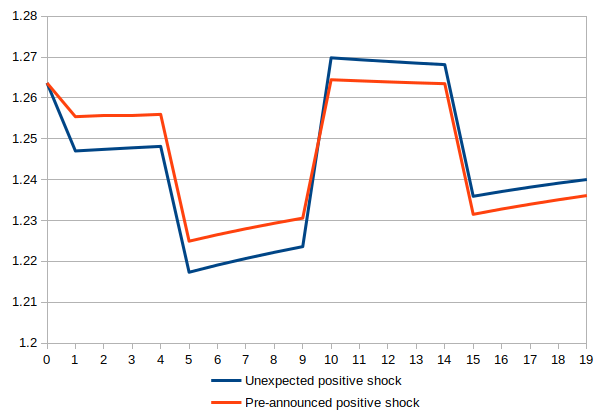
\includegraphics[width=11cm]{figures/consumption_unexpected.png}
\end{frame}




\section[Extended path]{Extended path}

\begin{frame}
  \frametitle{Extended path (EP) algorithm: idea}
  \begin{witemize}
    \item Idea: use the previous method to simulate a \emph{rational
      expectations} (RE) model (\textit{i.e.} with stochastic shocks that can
    happen at every period)\ldots
    \item \ldots but under the simplifying assumption that agents believe economy will not be perturbed in the future (i.e.\ future shocks are at steady state $u=0$), and do not update their belief when observing shocks\\
    $\rightarrow$ solve an approximation to the true RE model
    \item Advantage: \textit{deterministic} nonlinearities fully taken into account
    \item Inconvenient: solution under certainty equivalence violates Jensen's inequality\\
    $\rightarrow$ e.g.\ no precautionary motive.
    \item If goal is to generate a time series, method is superior to first-order perturbation (which is also certainty
    equivalent but ignores deterministic nonlinearities)
    \item Method introduced by \textcite{FairTaylor1983}
  \end{witemize}
\end{frame}

\begin{frame}
  \frametitle{Extended path (EP) algorithm}
  \begin{itemize}

    \item Algorithm
          \begin{enumerate}
            \item $H \leftarrow$ Set the horizon of the perfect foresight (PF) model
            \item $(y, u) \leftarrow$ Compute steady state of the model
            \item $y_0 \leftarrow$ Choose an initial condition for the endogenous variables
            \item \texttt{for} $t=1$ \texttt{to} $T$
            \item \hspace{2mm} $u_t  \leftarrow$ Draw random shocks for the current period
            \item \hspace{2mm} $y_t \leftarrow$ Solve a PF with:
                  \begin{itemize}
                    \item Initial condition: $y_{t-1}$ computed in previous iteration
                    \item Terminal condition: $y_{t+H}=y$
                    \item Shocks: $u_t$ just drawn and $u_{t+s}=u$ (for $s>0$)
                  \end{itemize}
            \item \texttt{end for}
          \end{enumerate}

    \item Implemented under the command \texttt{extended\_path} (with option
          \texttt{order=0}, which is the default)
    \item Option \texttt{periods} controls $T$
    \item Option \texttt{solver\_periods} controls $H$ (defaults to 200)
  \end{itemize}
\end{frame}

\begin{frame}[fragile]{Extended path: Dynare example}{\texttt{rbc\_ep.mod}}
  \begin{minted}{c++}
...
// Declare shocks as in a stochastic setup
shocks;
  var epsilon;
  stderr 0.02;
end;

extended_path(periods=300);

// Plot 20 first periods of consumption
ic = varlist_indices('c', M_.endo_names);
plot(oo_.endo_simul(ic, 1:21));
\end{minted}
\end{frame}

\begin{frame}
  \frametitle{Stochastic extended path (SEP)}
  \begin{witemize}
    \item Idea: generalize the extended path method to take into account
    \textit{some} future uncertainty
    \item Approximate rational expectations problem by one where agents at time $t$,
    \begin{itemize}
      \item know that there will be stochastic shocks in periods
            $t+1$ to $t+k$
      \item but assume no more shocks in periods after $t+k$
    \end{itemize}
    \item $k$ measures degree of future uncertainty taken into
    account
    \item The larger $k$, the closer we get to the true RE model (which corresponds to $k = +\infty$)
    \item Note: (plain) extended path (\texttt{order=0}) corresponds to $k=0$
    \item Additional approximation: probability distribution about future
    uncertainty is simplified using discrete numerical integration
    (\textit{a.k.a.} quadrature)
  \end{witemize}
\end{frame}

\begin{frame}
  \frametitle{Gauss-Hermite quadrature (univariate)}
  \begin{witemize}
    \item Let $X\sim N(0,\sigma_x^2)$ and suppose we need  to evaluate
    $\mathbb E  [\varphi(X)]$, where  $\varphi$ is a continuous function
    \item By definition we have:
    {\small\begin{equation}
      \mathbb E [\varphi(X)] =  \frac{1}{\sigma_x\sqrt{2\pi}}\int_{-\infty}^{\infty} \varphi(x)e^{-\frac{x^2}{2\sigma^2_x}}\mathrm dx
    \end{equation}
    }
    \item Integral can be approximated by a finite sum
    using Gauss-Hermite quadrature formula at order $n$:
    {\small
    \begin{equation}
      \int_{-\infty}^{\infty} \varphi(z)e^{-z^2}\mathrm dz \approx \sum_{i=1}^n\omega_i \varphi(z_i) \: ,
    \end{equation}
    }
    where $z_i$ ($i=1,\dots,n$) are the roots of an $n$th order Hermite  polynomial, and the weights  $\omega_i>0$ sum up to  one (variable change: $x_i  = \frac{z_i}{\sigma_x\sqrt{2}}$)
    \item The higher $n$, the better the approximation
  \end{witemize}
\end{frame}


\begin{frame}
  \frametitle{Gauss-Hermite quadrature (multivariate)}
  \begin{itemize}
    \item Let $X$ be a $p$-dimensional multivariate Gaussian random variable with mean zero and unit variance, and suppose we need to evaluate
            {\small\begin{equation}
                \mathbb E [\varphi(X)] =  (2\pi)^{-\frac{p}{2}}\int_{\mathbb R^{p}} \varphi(\mathbf{x})e^{-\frac{1}{2} \mathbf{x}'\mathbf{x}}\mathrm d\mathbf{x}
              \end{equation}
            }
    \item Let $\{(\omega_i,z_i)\}_{i=1}^n$ be the weights and nodes of an order $n$ univariate Gauss-Hermite quadrature
    \item This integral can be approximated using a tensor grid:
          {\small\begin{equation}
            \int_{\mathbb R^{p}} \varphi(\mathbf{z})e^{-\mathbf{z}'\mathbf{z}}\mathrm d\mathbf{z} \approx \sum_{i_1,\dots,i_p=1}^n\omega_{i_1}\dots\omega_{i_p} \varphi(z_{i_1},\dots,z_{i_p})
          \end{equation}
          }
    \item \textbf{Curse of dimensionality 1:} number of terms in
          sum grows exponentially with number of shocks
  \end{itemize}
\end{frame}

\begin{frame}[fragile]
  \frametitle{Other numerical integration rules}
  \begin{witemize}
    \item Default: use multivariate Gaussian quadrature to approximate the expected terms
    \item To cope with \textbf{curse of dimensionality 1}, can consider other numerical integration approaches:
    \begin{witemize}
      \item[--] Cubature (order 3 or 5)\\
            Set \verb+options_.ep.IntegrationAlgorithm+ to \verb+'Stroud-Cubature-3'+\\
            or \verb+'Stroud-Cubature-5'+
      \item[--] Unscented transform\\
            Set \verb+options_.ep.IntegrationAlgorithm+ to \verb+'Unscented' +
    \end{witemize}
    $\rightarrow$ rely on smaller number of nodes which does
    not grow exponentially with number of innovations
    \item Unfortunately, there is another curse of dimensionality
  \end{witemize}
\end{frame}


\begin{frame}
  \frametitle{Forward history}
  \framesubtitle{One shock, three quadrature nodes, order two SEP ($k=2$)}
  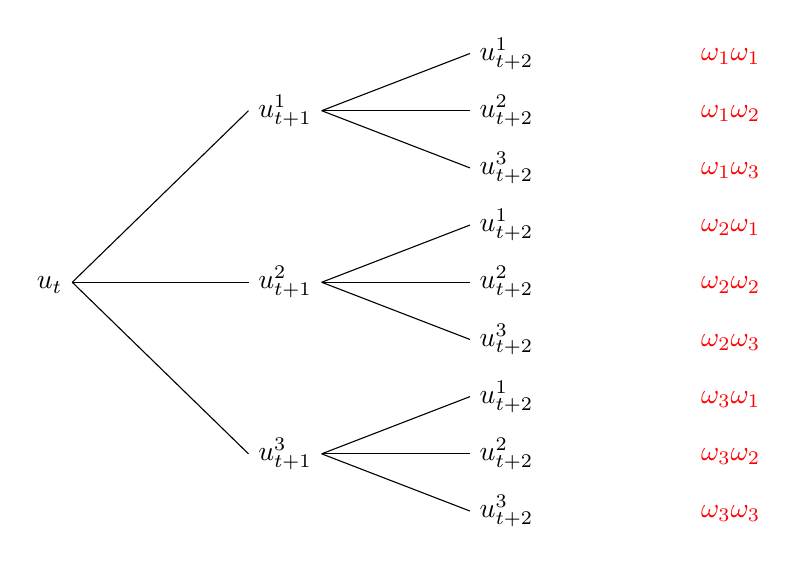
\begin{tikzpicture}
    \tikzset{grow'=right,level distance=80pt}
    \tikzset{execute at begin node=\strut}
    \tikzset{every tree node/.style={anchor=base west}}
    \Tree [.$u_t$ [.$u^1_{t+1}$ [.$u^1_{t+2}$  \edge[white]; \color{red}{$\omega_1\omega_1$} ]
    [.$u^2_{t+2}$   \edge[white]; \color{red}{$\omega_1\omega_2$} ]
    [.$u^3_{t+2}$  \edge[white];
    \color{red}{$\omega_1\omega_3$} ]]
    [.$u^2_{t+1}$ [.$u^1_{t+2}$  \edge[white]; \color{red}{$\omega_2\omega_1$} ]
    [.$u^2_{t+2}$   \edge[white]; \color{red}{$\omega_2\omega_2$} ]
    [.$u^3_{t+2}$  \edge[white];
    \color{red}{$\omega_2\omega_3$} ]]
    [.$u^3_{t+1}$ [.$u^1_{t+2}$  \edge[white]; \color{red}{$\omega_3\omega_1$} ]
    [.$u^2_{t+2}$   \edge[white]; \color{red}{$\omega_3\omega_2$} ]
    [.$u^3_{t+2}$  \edge[white]; \color{red}{$\omega_3\omega_3$} ]]
    ]
  \end{tikzpicture}
  $\rightarrow$ The tree of histories grows exponentially
\end{frame}

\begin{frame}
  \frametitle{Fishbone integration}
  \begin{witemize}
    \item We can prune the tree of forward histories by removing low probability branches...
    \item Or by considering that innovations, say, at time $t+1$ and $t+2$ are unrelated variables
    \item {\color{gray} Analogy with a good  at different periods in an intertemporal general equilibrium model.}\newline
    \item If we have $n_u$ innovations and if agents perceive uncertainty for the following $k$  periods, we consider integration problem involving $n_u \times k$ unrelated variables
    \item Use two points Cubature rule to compute the integral (unscented transform with $\kappa=0$)\\
    $\rightarrow$ complexity of integration problem grows linearly with $n_u$ or $k$
  \end{witemize}
\end{frame}

\begin{frame}
  \frametitle{Fishbone history (one shock, two nodes, order three SEP)}
  \begin{center}
    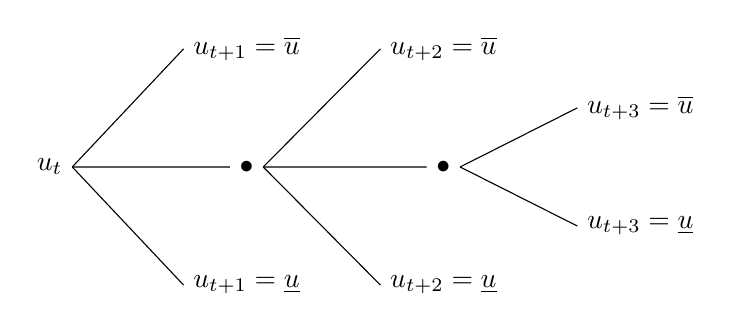
\begin{tikzpicture}[grow=right,level distance=2.5cm]
      \node {$u_t$}
      child {
          node {$u_{t+1}=\underline{u}$}
        }
      child {
          node {$\bullet$}
          child {
              node {$u_{t+2}=\underline{u}$}
            }
          child {
              node {$\bullet$}
              child {
                  node {$u_{t+3}=\underline{u}$}
                }
              child {
                  node {$u_{t+3}=\overline{u}$}
                }
            }
          child {
              node {$u_{t+2}=\overline{u}$}
            }
        }
      child {
          node {$u_{t+1}=\overline{u}$}
        };
    \end{tikzpicture}
  \end{center}
\end{frame}


\begin{frame}
  \frametitle{Stochastic extended path algorithm}
  \algsetup{
    linenosize=\small,
    linenodelimiter=.
  }
  \begin{algorithm}[H]
    \caption{Stochastic Extended path algorithm}
    \label{alg:ep}
    \begin{algorithmic}[1]
      \STATE $H \leftarrow$ Set the horizon of the \emph{stochastic} perfect foresight (SPF) models.
      \STATE $(x^\star, y^\star) \leftarrow$ Compute steady state of the model.
      \STATE $\{(\omega_i,\mathfrc u_i)\}_{i=1}^m \leftarrow$ Get weights and nodes for numerical integration
      \STATE $(s_0, x_1) \leftarrow$ Choose an initial condition for the state variables
      \FOR{$t=1$ to $T$}
      \STATE $u_t  \leftarrow$ Draw random shocks for the current period
      \STATE $(y_t,x_{t+1},s_t) \leftarrow$ Solve a SPF model with $y_{t+H+1}=y^{\star}$
      \ENDFOR
    \end{algorithmic}
  \end{algorithm}
\end{frame}

\begin{frame}
  \frametitle{Stochastic extended path (SEP) (continued)}
  \begin{witemize}
    \item SEP algorithm is similar to EP, but instead of solving
    a perfect foresight (PF) problem for each period, a larger problem is
    solved:
    \begin{itemize}
      \item equations determining future variables are replicated as many
            times as there are branches on the tree of history;
      \item Gauss-Hermite quadrature is used to compute expectations over those future variables
    \end{itemize}
    \item We face two curses of dimensionality (exponential complexity growth):
    \begin{itemize}
      \item Stochastic order ($k$)
      \item Number of shocks
    \end{itemize}
    \item In practice, only feasible for small $k$ and small number of shocks
    \item SEP triggered with option \texttt{order=k} of \texttt{extended\_path}
    command
    \item NB: currently no interface for controlling the number of nodes for the
    Gauss-Hermite quadrature\\
    $\rightarrow$ has to be directly set in the
    \texttt{options\_} structure
  \end{witemize}
\end{frame}

%\section{Dealing with nonlinearities using higher order approximation of stochastic models}
%
%\begin{frame}
%  \frametitle{Local approximation of stochastic models}
%  The general problem:
%
%  \begin{equation*}
%    \mathbb{E}_t f(y_{t+1},y_t,y_{t-1},u_t)=0
%  \end{equation*}
%  \begin{description}
%  \item[$y$]: vector of endogenous variables
%  \item[$u$]: vector of exogenous shocks
%  \end{description}
%  with:
%  \begin{eqnarray*}
%    \mathbb{E}(u_t) &=& 0\\
%    \mathbb{E}(u_tu_t') &=& \Sigma_u\\
%    \mathbb{E}(u_tu_s') &=& 0\;\text{ for } t\neq s
%  \end{eqnarray*}
%
%\end{frame}
%
%\begin{frame}
%  \frametitle{What is a solution to this problem?}
%  \begin{itemize}
%  \item  A solution is a policy function of the form:
%  \begin{equation*}
%    y_t = g\left(y_{t-1},u_t,\sigma\right)
%  \end{equation*}
%  where $\sigma$ is the \emph{stochastic scale} of the problem and:
%  \begin{equation*}
%    u_{t+1} = \sigma\,\varepsilon_{t+1}
%  \end{equation*}
%  \item The policy function must satisfy:
%    \begin{equation*}
%      \mathbb{E}_t f\left(g\left(
%          g\left(y_{t-1},u_t,\sigma\right),u_{t+1},\sigma\right), g\left(y_{t-1},u_t,\sigma\right),y_{t-1},u_t\right)=0
%    \end{equation*}
%  \end{itemize}
%\end{frame}
%
%\begin{frame}
%  \frametitle{Local approximations}
%
%  \begin{align*}
%    \hat{g}^{(1)}\left(y_{t+1},u_t,\sigma\right) &= \bar y + g_y\hat y_{t-1} +
%    g_u u_t\\
%    \hat{g}^{(2)}\left(y_{t+1},u_t,\sigma\right) &= \bar y + {\red \frac{1}{2} g_{\sigma\sigma}}+g_y\hat y_{t-1} +
%    g_u u_t\\
%    &\quad + \frac{1}{2}\left(g_{yy}\left(\hat y_{t-1}\otimes\hat
%        y_{t-1}\right)+g_{uu}\left(u_t\otimes u_t\right)\right)\\
%    &\quad +g_{yu}\left(\hat y_{t-1}\otimes u_t\right)\\
%    \hat{g}^{(3)}\left(y_{t+1},u_t,\sigma\right) &= \bar y + {\red \frac{1}{2}
%      g_{\sigma\sigma}+ \frac{1}{6}
%      g_{\sigma\sigma\sigma}+\frac{1}{2}g_{\sigma\sigma y}\hat
%      y_{t-1}+\frac{1}{2}g_{\sigma\sigma u} u_t}\\
%    & \quad +g_y\hat y_{t-1} +
%    g_u u_t + \ldots
%  \end{align*}
%\end{frame}
%
%\begin{frame}[fragile]
%  \frametitle{Breaking certainty equivalence (1/2)}
%  The combination of future uncertainty (future shocks) and nonlinear
%  relationships makes for precautionary motives or risk premia.
%  \begin{itemize}
%  \item 1\textsuperscript{st} order: certainty equivalence; today's decisions don't
%    depend on future uncertainty
%  \item 2\textsuperscript{nd} order:
%    \begin{align*}
%      \hat{g}^{(2)}\left(y_{t+1},u_t,\sigma\right) &= \bar y + {\red \frac{1}{2} g_{\sigma\sigma}}+g_y\hat y_{t-1} +
%      g_u u_t\\
%      &\quad + \frac{1}{2}\left(g_{yy}\left(\hat y_{t-1}\otimes\hat
%          y_{t-1}\right)+g_{uu}\left(u_t\otimes u_t\right)\right)\\
%      &\quad +g_{yu}\left(\hat y_{t-1}\otimes u_t\right)
%    \end{align*}
%    Risk premium is a constant: ${\red \frac{1}{2} g_{\sigma\sigma}}$
%  \end{itemize}
%\end{frame}
%
%\begin{frame}
%  \frametitle{Breaking certainty equivalence (2/2)}
%  \begin{itemize}
%  \item 3\textsuperscript{rd} order:
%    \begin{multline*}
%      \hat{g}^{(3)}\left(y_{t+1},u_t,\sigma\right) = \bar y + {\red \frac{1}{2}
%        g_{\sigma\sigma}+ \frac{1}{6}
%        g_{\sigma\sigma\sigma}+\frac{1}{2}g_{\sigma\sigma y}\hat
%        y_{t-1}+\frac{1}{2}g_{\sigma\sigma u} u_t}\\
%      +g_y\hat y_{t-1} +
%      g_u u_t + \ldots
%    \end{multline*}
%    Risk premium is linear in the state variables:
%    \begin{equation*}
%      {\red \frac{1}{2}
%        g_{\sigma\sigma}+ \frac{1}{6}
%        g_{\sigma\sigma\sigma}+\frac{1}{2}g_{\sigma\sigma y}\hat
%        y_{t-1}+\frac{1}{2}g_{\sigma\sigma u} u_t}
%    \end{equation*}
%  \end{itemize}
%\end{frame}
%
%\begin{frame}[fragile]
%  \frametitle{The cost of local approximations}
%  \begin{enumerate}
%    \item High order approximations are accurate around the steady state, and
%      more so than lower order approximations
%    \item But can be totally wrong far from the steady state (and may be more
%      so than lower order approximations)
%    \item Error of approximation of a solution $\hat{g}$, at a given point of
%      the state space $(y_{t-1}, u_t)$:
%    \begin{equation*}
%      \mathcal{E}\left(y_{t-1},u_t\right) =
%      \mathbb{E}_t f\left(\hat g\left(\hat
%          g\left(y_{t-1},u_t,\sigma\right),u_{t+1},\sigma\right),\hat g\left(y_{t-1},u_t,\sigma\right),y_{t-1},u_t\right)
%    \end{equation*}
%    \item Necessity for pruning
%  \end{enumerate}
%\end{frame}
%
%\begin{frame}
%  \frametitle{Approximation of occasionally binding constraints with
%    penalty functions}
%
%  The investment positivity constraint is translated into a penalty on the welfare:
%  \begin{equation*}
%    \max_{\{c_{t+j},\ell_{t+j},k_{t+j}\}_{j=0}^{\infty}}
%    \sum_{j=0}^{\infty}\beta^j
%    u(c_{t+j},\ell_{t+j})+h\cdot\log(i_{t+j})
%  \end{equation*}
%  s.t.
%  \begin{gather*}
%      y_t = c_t + i_t\\
%       y_t = A_tf(k_{t-1},\ell_t)\\
%       k_t = i_t + (1-\delta)k_{t-1}\\
%       A_{t} = {A^{\star}}e^{a_{t}}\\
%       a_{t} = \rho\, a_{t-1} + \varepsilon_t
%     \end{gather*}
%     where the technology ($f$) and the preferences ($u$) are as
%  before, and $h$ governs the strength of the penalty (\emph{barrier parameter})
%\end{frame}


\end{document}
